\documentclass[12pt]{fithesis2}

% ===== LOADING PACKAGES =====
% language settings, main documnet language last
\usepackage[english]{babel}
% enabling new fonts support (nicer)
\usepackage{lmodern}
% setting input encoding
\usepackage[utf8]{inputenc}
% setting output encoding
\usepackage[T1]{fontenc}
% fithesis2 requires csquotes
\usepackage{csquotes}

\usepackage{subfig}
\usepackage{graphicx}
\usepackage{kpfonts}
\usepackage[labelfont=bf, margin=0.5cm, font=small, skip=1pt]{caption}
\usepackage{stmaryrd}
\usepackage{mathtools}
\usepackage[usenames, dvipsnames]{color}
\usepackage{esvect}
\usepackage{url}
\usepackage{dsfont}
\usepackage{color}
\usepackage{tikz}
\usepackage{pythonhighlight}
\usepackage[hidelinks]{hyperref}
\usepackage{bbm}
\usepackage{braket}

\newcounter{counter}[section]
\renewcommand{\thecounter}{\thesection.\arabic{counter}}
\newenvironment{definition}[1]{\bigskip\refstepcounter{counter}\noindent\textbf{Definition \thecounter } \textit{#1} \par\nopagebreak}{\bigskip}
\newenvironment{example}[1]{\bigskip\refstepcounter{counter}\noindent\textbf{Example \thecounter} \textit{#1} \par\nopagebreak}{\bigskip}
\newenvironment{notation}{\bigskip\refstepcounter{counter}\noindent\textbf{Notation \thecounter}\par\nopagebreak}{\bigskip}
\newenvironment{proof}{\bigskip\refstepcounter{counter}\noindent\textbf{Proof \thecounter}\par\nopagebreak}{\bigskip}
\newenvironment{runningExample}[1]{\bigskip\refstepcounter{counter}\noindent\textbf{Running example \thecounter} \textit{#1} \par\nopagebreak}{\bigskip}
\newenvironment{theorem}{\bigskip\refstepcounter{counter}\noindent\textbf{Theorem \thecounter }\par\nopagebreak}{\bigskip}
\newenvironment{remark}{\bigskip\refstepcounter{counter}\noindent\textbf{Remark \thecounter }\par\nopagebreak}{\bigskip}

\newcommand\mdoubleplus{\mathbin{+\mkern-7mu+}}
\newcommand*\arc{{\fontfamily{pbk}\fontseries{db}\selectfont+}}
\newcommand\myeq{\stackrel{\mathclap{\scriptsize\mbox{def}}}{\Leftrightarrow}}
\newcommand*{\QEDA}{\hfill\ensuremath{\blacksquare}}%

\definecolor{gray}{rgb}{0.4,0.4,0.4}
\definecolor{graybright}{rgb}{0.5,0.5,0.5}
\definecolor{darkblue}{rgb}{0.0,0.0,0.6}
\definecolor{cyan}{rgb}{0.0,0.6,0.6}

\lstset{
  basicstyle=\ttfamily,
  columns=fullflexible,
  showstringspaces=false,
  commentstyle=\color{gray}\upshape
}

\lstdefinelanguage{XML}
{
  morestring=[b]",
  morestring=[s]{>}{<},
  morecomment=[s]{<?}{?>},
  stringstyle=\color{black},
  identifierstyle=\color{darkblue},
  keywordstyle=\color{cyan},
  morekeywords={xmlns,version,type}% list your attributes here
}

\usetikzlibrary{fit, hobby}
\usetikzlibrary{chains}
\usetikzlibrary{arrows,positioning,decorations.markings} 
\usetikzlibrary{decorations.pathmorphing}
\tikzset{snake it/.style={decorate, decoration=snake}}


\tikzset{
    myarrow/.style={
        decoration={markings,mark=at position 1 with {\arrow[scale=1]{>}}},
        postaction={decorate},
        >=stealth
    }
}

\definecolor{mydarkgreen}{RGB}{48, 129, 7}

% uncomment in case of \subsubsection usage
% \usepackage{titlesec}
% \titleformat{\subsubsection}{}{\thesubsubsection}{1em}{\bfseries}

% FI THESIS settings
\thesistitle{Formal biochemical space for specification and analysis of biochemical processes}
\thesissubtitle{Master thesis}
\thesisstudent{Matej Troják}
\thesiswoman{false}
\thesisfaculty{fi}
\thesisyear{autumn 2017}
\thesisadvisor{RNDr.\ David Šafránek,\ Ph.D.}
\thesislang{en}

% ===== BEGIN DOCUMENT =====
\begin{document}

\FrontMatter
\ThesisTitlePage

\begin{ThesisDeclaration}
\DeclarationText
\AdvisorName
\end{ThesisDeclaration}

\begin{ThesisThanks}
Many thanks to you all.
\end{ThesisThanks}

\begin{ThesisAbstract}
Abstract
\end{ThesisAbstract}

\begin{ThesisKeyWords}
key words
\end{ThesisKeyWords}

\MainMatter
\tableofcontents

\chapter{Introduction}

\chapter{Background}

In this chapter, we introduce all relevant terms which will be used in the thesis. Namely, we give an introduction to rule-based modelling and compare it to usual reaction-based approach. Then we describe typical representatives of the rule-based languages and highlight their key features. We also introduce Comprehensive Modeling Platform with its core parts and provide motivation for Biochemical Space as a key feature of the platform.

\section{Rule-based modelling}
\label{Rule-based basics}

Modelling complex systems in biology, such as individual cells, is necessary with respect to their complexity and size. The more complex the system is, the harder it is to describe it formally. The typical approach in modelling is using chemical reactions or ordinary differential equations~\cite{coddington1955theory}. The general problem with these approaches is that they require to enumerate all interacting objects and interactions themselves. However, this number is often too high to be effectively processed. Rule-based modelling offers a solution for this problem. It is a natural extension of reaction-based approach. Instead of operating with objects, we operate with \emph{types} of objects. The semantics of the model are defined via \emph{rules} on the given types. Typically, rule-based models are more concise.

There are multiple approaches to rule-based modelling, but all of them match in principle described above.

We represent a rule-based model $\mathds{M}$ as a set of rules and an initial solution of interacting objects. We understand solution as a mixture of individual objects which are randomly distributed (Fig.~\ref{solutions:fig}a). Therefore, we cannot assign them any order and we do not see as multisets. From biological perspective, this representation of solution is as close as is possible to the reality while preserving conciseness.

The rules are patterns which describe behavior of groups of objects. A rule has form of an abstract chemical reaction, where substrates and products take place. The difference is that reaction only operates on particular objects, while in rule groups of objects are interacting. Therefore, a reaction can be seen as a special case of a rule (Fig.~\ref{rules:fig}), where the type represents exactly one object.

\begin{figure}[!h]
\begin{center}
\subfloat[]{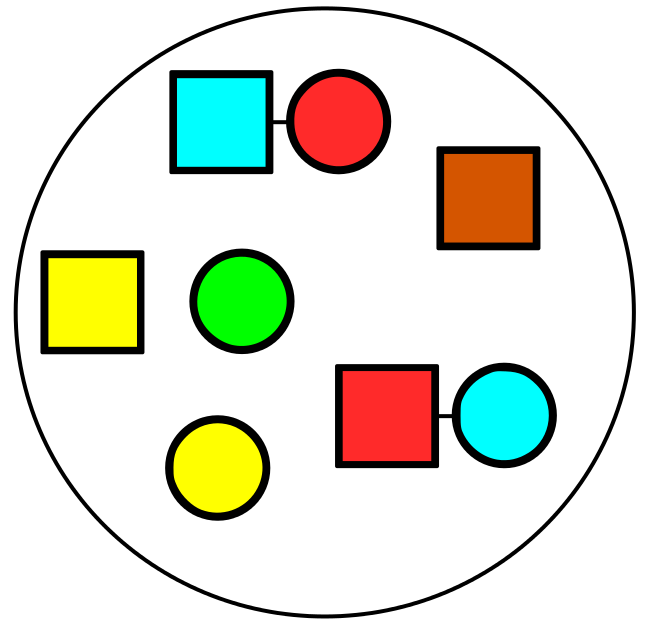
\includegraphics[scale=0.23]{pics/solution_first}\label{sol:s1}}
\hspace*{1cm}
\subfloat[]{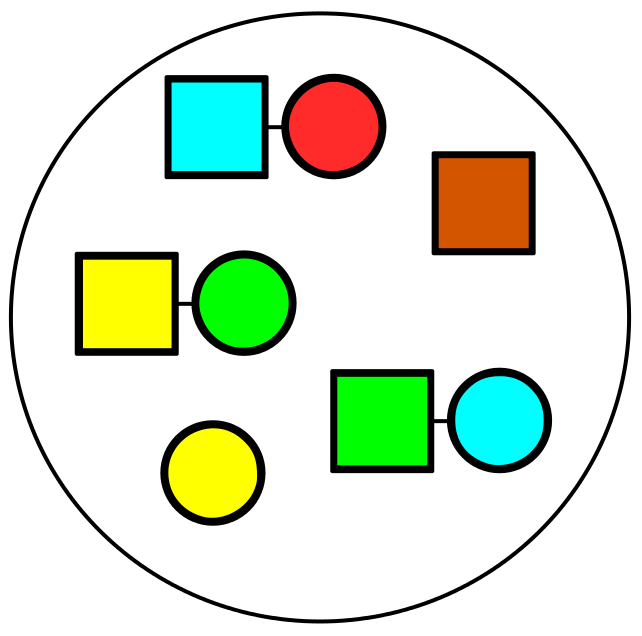
\includegraphics[scale=0.23]{pics/solution_second}\label{sol:s2}}
\caption{\textbf{Examples of solutions}. \textbf{(a)} An example of graphical representation of a solution. \textbf{(b)} Updated solution after rules from Fig.~\ref{rules:fig} were applied. The first rule \textit{(a)} was applied on the yellow \raisebox{-0.02cm}[0cm]{{\large $\square$}} and green $\bigcirc$ and produced yellow-green complex \raisebox{-0.02cm}[0cm]{{\large $\square$}}--$\bigcirc$. Note there are more options how the rule could be mapped -- each combination of free \raisebox{-0.02cm}[0cm]{{\large $\square$}} and $\bigcirc$. The second rule \textit{(b)} was applied on red-cyan complex \raisebox{-0.02cm}[0cm]{{\large $\square$}}--$\bigcirc$ where the color of \raisebox{-0.02cm}[0cm]{{\large $\square$}} was changed from red to green. The third rule \textit{(c)} couldn't be applied because there is no such complex with yellow $\bigcirc$. }
\label{solutions:fig}
\end{center}
\end{figure}

\begin{figure}[!h]
\begin{center}
\begin{minipage}[l]{0.1\textwidth}
    \textbf{(a)}
  \end{minipage}
  \begin{minipage}[r]{0.6\textwidth}
    {\hspace*{0.8cm}
\includegraphics[scale=0.2]{pics/rule_complex}}
\end{minipage}

\begin{minipage}[l]{0.1\textwidth}
    \textbf{(b)}
  \end{minipage}
  \begin{minipage}[r]{0.6\textwidth}
    {\hspace*{1.35cm}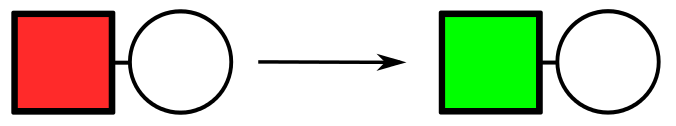
\includegraphics[scale=0.2]{pics/rule_change}}
\end{minipage}

\begin{minipage}[l]{0.1\textwidth}
    \textbf{(c)}
  \end{minipage}
  \begin{minipage}[r]{0.6\textwidth}
    {\hspace*{1.3cm}
\includegraphics[scale=0.2]{pics/rule_diss}}
\end{minipage}
\caption{\textbf{Examples of rules}. Rule \textbf{(a)}: a \raisebox{-0.02cm}[0cm]{{\large $\square$}} and a $\bigcirc$ can form a complex \raisebox{-0.02cm}[0cm]{{\large $\square$}}--$\bigcirc$ regardless their colors. Rule \textbf{(b)}: a \raisebox{-0.02cm}[0cm]{{\large $\square$}} is allowed to change its color from red to green only if is in a complex with a $\bigcirc$ regardless its color. Rule \textbf{(c)}: the rule can disassemble the complex only if the $\bigcirc$ is yellow.}
\label{rules:fig}
\end{center}
\end{figure}

The rule is mapped on a solution. Then it can be applied and a new solution is produced. The mapping is not always successful (Fig.~\ref{solutions:fig}, application of rule \textit{c}). %By repeating map-apply action, we obtain a \textit{Labelled transition system} $\mathcal{L}$ (Definition~\ref{lts}).

The mapping of a rule on a solution can be understood as a particular moment when the objects in the solution have just the conformation suitable for the rule and therefore the rule can be applied. Since the distribution of objects is random, we can assume a sequence of objects needed for rule (if there are such objects) is always available.

\begin{figure}[!h]
\begin{center}
\begin{minipage}[l]{0.1\textwidth}
    \textbf{(a)}
  \end{minipage}
  \begin{minipage}[r]{0.6\textwidth}
    {\hspace*{1.3cm}
\includegraphics[scale=0.2]{pics/rule_complex}}
\end{minipage}

\begin{minipage}[l]{0.1\textwidth}
    \textbf{(b)}
  \end{minipage}
  \begin{minipage}[r]{0.6\textwidth}
    {\hspace*{1.3cm}
\includegraphics[scale=0.2]{pics/rule_complex_mapped}}
\end{minipage}

\begin{minipage}[l]{0.1\textwidth}
    \textbf{(c)}
  \end{minipage}
  \begin{minipage}[r]{0.6\textwidth}
    {\hspace*{1.3cm}
\includegraphics[scale=0.2]{pics/rule_reaction}}
\end{minipage}
\caption{\textbf{Example of a map-apply action}. As a solution, we use solution \textit{(a)} from Fig.~\ref{solutions:fig}. \textbf{(a)} Rule can be mapped on a \raisebox{-0.02cm}[0cm]{{\large $\square$}} and a $\bigcirc$ regardless their colors and form a complex \raisebox{-0.02cm}[0cm]{{\large $\square$}}--$\bigcirc$.  \textbf{(b)} Let's choose yellow \raisebox{-0.02cm}[0cm]{{\large $\square$}} and green $\bigcirc$ from our solution. The rule was mapped on chosen objects and they were assigned to the left-hand-side of the rule. \textbf{(c)} The rule was applied and new object (yellow-green complex \raisebox{-0.02cm}[0cm]{{\large $\square$}}--$\bigcirc$) was created. We obtained the reaction describing the particular action which has just happened.}
\label{map-apply:fig}
\end{center}
\end{figure}

The mapping can also be seen as assigning particular objects from the solution to types on the left-hand-side of the rule. The rule application then represents the change of the mapped objects to new objects according to the right-hand-side of the rule (i.e., particular objects are assigned to the right-hand-side). As a by-product, we obtain an instance of the rule -- a reaction (Fig.~\ref{map-apply:fig}). %This is how we construct the set of labels (reactions) $A$ in the LTS $\mathcal{L}$.

Since this kind of graphical representation is not very suitable for machine processing and analyses, we define a formal language which is built on principles described in this chapter.

\section{Rule-based vs. reaction-based modelling}

A rule is a generalised reaction (Figure~\ref{reaction_vs_rule}). This is how the difference can be characterised. From the application point of view, reaction can be applied on a solution only in a particular way whilst rule can be applied in multiple ways. It allows to write models where many similar processes might occur with rules, by defining a pattern in which the action can happen. Since there might be many features we need to express, there are several languages focusing on different level of details.

\begin{figure}[!h]
\begin{center}
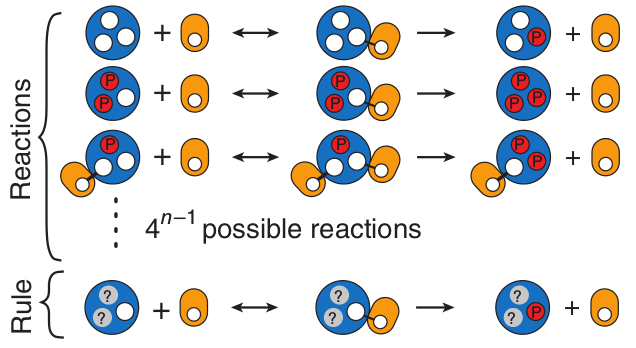
\includegraphics[scale=0.5]{pics/reaction_vs_rule}
\end{center}
\caption{Graphical comparison of rule-based and reaction-based approaches. There can be seen combinatorial explosion in number of possible particular interactions (reactions), which can be depicted in a few simple rules.}\label{reaction_vs_rule}
\end{figure}

Analysis of rules directly is not the best choice. The main reason are \emph{side effects}, which might happen during rule application. These side effects differ from language to language. There is no such thing for reaction because the entire context is enumerated explicitly. Therefore, we cannot directly know how exactly the rule will be used.

The rule and reaction differ in level of abstraction. In this context we mean how stringent it is, not what sort of features particular language uses. This is universal attribute for all rule-based languages -- the rule is always more abstract than its instance -- a reaction. The analysis of such abstract object statically is a challenge. The reason is that most of the structural information is encoded in rules implicitly. Explicit data are more suitable for static analysis.

\section{Rule-based languages}
\label{rule_based_languages}

There are several rule-based languages dedicated for modeling of biological systems. Each of them uses different features and abstractions. In this chapter, we will highlight the key features for some representatives of them.

\subsection{Kappa}
\label{kappa}

The Kappa language~\cite{kappa_formal} was developed for modeling of protein-protein interactions. The key structures used in the language are \textit{agents} with \textit{binding sites}, which allow formation of \emph{bonds} between the agents. Each binding site must be unique with at most one bond. Each site can occur in one of several pre-defined states.

The Kappa \textit{rules} are changing properties of the agents. Particularly, it might add/delete/change a bond or a state of one or multiple agents at once. The rules are just patterns where on both sides is a sequence of agents delimited by a comma. Same as all the other rule-based languages, when some context is not relevant, the just omit it. Example of a rule is in Figure~\ref{kappa-rule}.

\begin{figure}[!h]
\begin{center}
\begin{tabular}{c l}
(a) & A(bsa$\sim$\{ u, p \}) ; B(bsb$\sim$\{ a, i \}) \\
(b) & A(bsa), B(bsb$\sim$a) $\rightarrow$ A(bsa!1), B(bsb$\sim$a!1) \\
\end{tabular}
\end{center}
\caption{Example of a Kappa rule. (a) Definition of associated agents. There are allowed two agents, A and B, both with a binding site which might occur in two possible states. (b) The rule itself. It defines creation of bond on the sites of agents A and B such that site of agent B must be in a active state. Note the context which has no importance for the interaction is omitted.}\label{kappa-rule}
\end{figure}

The general problem they have to handle in Kappa is too detailed description. For biological systems as defined in Chapter~\ref{Rule-based basics}, it might be often hard to deal with all the bonds, especially in cases when we do not need such details.

\subsection{BioNetGen Language}
\label{bngl}

BioNetGen Language (BNGL) \cite{BNGL} is very similar to Kappa language and also has similar disadvantages. There are a few general differences: 

\begin{enumerate}
	\item it is allowed to define multiple binding sites with same name for an agent,
	\item one binding site is allowed to have multiple bonds,
	\item in the rules BNGL uses `+' and `.' for expressing reaction complex and complex of agents respectively.
\end{enumerate}

Example of a rule is given in Figure~\ref{bngl-rule}.

\begin{figure}[!h]
\begin{center}
\begin{tabular}{c l}
(a) & A(bsa$\sim$u$\sim$p) \\
  & B(bsb$\sim$a$\sim$i) \\
(b) & A(bsa) + B(bsb$\sim$a) $\rightarrow$ A(bsa!1).B(bsb$\sim$a!1) \\
\end{tabular}
\end{center}
\caption{Example of a BGNL rule. (a) Definition of associated agents. There are allowed two agents, A and B, both with a binding site which might occur in two possible states. (b) The rule itself. Note the A and B agents must first create \emph{reaction complex} denoted with `+' (i.e., they must be close to each other) and then they create \emph{complex of agents} denoted as `.' (i.e., they are physically connected).}\label{bngl-rule}
\end{figure}

\subsection{Chromar}

The Chromar language~\cite{honorato2017chromar} allows to define attributes for agents and range them over pre-defined domains. The qualitative semantics are given by rule match on multisets composed from these agents producing reaction. It is followed by standard application of the reaction (in manner of multiset operations). The language is very useful when creating a model where we need to create new distinct objects and control population of these objects.

Embedding this language to functional programming language Haskell increases its expressive power while making the ability of some analysis more expensive. Moreover, a user needs to understand Haskell (at least its basics) in order to use Chromar.

It is important to highlight a feature of stochastic semantics which this language offers. Compared to other rule-based languages, it is capable of specifying rates for individual reactions inherited from the rule (Figure~\ref{chromar_rule}). It is allowed by variable value bindings and type-determination between left- and right-hand-side of the rule.

\begin{figure}[!h]
\begin{center}
A(a = x), A(a = y) $\xrightarrow[]{\text{f(x,y)}}$ A(a = x + y), A(a = y - 1) [g(x, y)]
\end{center}
\caption{Example of a Chromar rule. Arithmetic operations can be used in order to change properties of individual agents. Moreover, a rate function $f$ and conditional function $g$ increase applicability and practical use of the rule.}\label{chromar-rule}\label{chromar_rule}
\end{figure}

However, when it comes to readability and presentation to the user, the language is not a best choice. All the biologically relevant terms such as states must be encoded to natural numbers.

\subsection{PySB}

The PySB language~\cite{Lopez646} works as a package in Python programming language. The definition of models directly in the code allows to use the full syntax of Python, what significantly increases expression power of PySB. On the other hand, it might be hard to follow abstraction which possible is this way and models themselves are hard to analyze. Moreover, the core of the language is made by translating to BGNL~\ref{bngl}. An example of a rule is given in Figure~\ref{pysb_rule}.

\begin{figure}[!h]
\begin{center}
\begin{python}
# Declare the monomers
Monomer('L', ['s'])
Monomer('R', ['s'])

# Declare the binding rule
Rule(L(s=None) + R(s=None) <> L(s=1) % R(s=1), kf, kr)
\end{python}
\end{center}
\caption{Example of a PySB rule. The rule describes creation of a bond between agents $\mathtt{R}$ and $\mathtt{L}$.}\label{PySB-rule}\label{pysb_rule}
\end{figure}

\subsection{SBML-multi package}

Systems Biology Markup Language (SBML)~\cite{hucka2003systems} is a standard established for systems biology. A SBML-multi package~\cite{zhang2015sbml} is able to describe all necessary rule-based features and therefore it is possible to export each such language in this format. It is the most suitable format for exchange and storage of the models but less for analysis and direct representation to the users (it is an XML format). It serves as intermediate language.

\begin{figure}[!h]
\lstset{language=XML}
\begin{lstlisting}[basicstyle=\tiny, frame=single]
<?xml version="1.0" encoding="UTF-8"?>
<sbml xmlns="http://www.sbml.org/sbml/level2" level="2" version="1">
  <model>
    <listOfCompartments>
      <compartment id="c" constant="true" multi:isType="true" />
      <compartment id="cc" constant="true" multi:isType="true">
        <multi:listOfCompartmentReferences>
          <multi:compartmentReference multi:id="cr1" multi:compartment="c" />
          <multi:compartmentReference multi:id="cr2" multi:compartment="c" />
        </multi:listOfCompartmentReferences>
      </compartment>
    </listOfCompartments>
    <multi:listOfSpeciesTypes>
      <multi:bindingSiteSpeciesType multi:id="stA" multi:compartment="c" />
      <multi:speciesType multi:id="stAA" multi:compartment="cc">
        <multi:listOfSpeciesTypeInstances>
          <multi:speciesTypeInstance multi:id="stiA1" multi:speciesType="stA"
            multi:compartmentReference="cr1" />
          <multi:speciesTypeInstance multi:id="stiA2" multi:speciesType="stA"
            multi:compartmentReference="cr2" />
        </multi:listOfSpeciesTypeInstances>
        <multi:listOfInSpeciesTypeBonds>
          <multi:inSpeciesTypeBond multi:bindingSite1="stiA1" multi:bindingSite2="stiA2" />
        </multi:listOfInSpeciesTypeBonds>
      </multi:speciesType>
    </multi:listOfSpeciesTypes>
    <listOfSpecies>
      <species id="spA" multi:speciesType="stA" compartment="c" ... />
      <species id="spAA" multi:speciesType="stAA" compartment="cc" ... />
    </listOfSpecies>
    <listOfReactions>
      <reaction id="reaction" ...>
        <listOfReactants>
          <speciesReference id="r1" species="spA" multi:compartmentReference="cr1" ... />
          <speciesReference id="r2" species="spA" multi:compartmentReference="cr2" ... />
        </listOfReactants>
        <listOfProducts>
          <speciesReference species="spAA" ... />
        </listOfProducts>
        ...
      </reaction>
      ...
    </listOfReactions>
  </model>
</sbml>
\end{lstlisting}
\caption{Example of a simple SBML-multi model. There are included SpeciesTypes, Species which belong to these types, and Reactions where those species are interacting.}\label{SBML_example}
\end{figure}

\section{Comprehensive Modeling Platform}
\label{cmp}

Comprehensive Modeling Platform (CMP)~\cite{cs2bio2013} is an online platform providing tools for public sharing, annotation, analysis, and visualization of dynamical models and \emph{wet-lab} experiments related to domain-specific systems. The platform is unique in integrating abstract mathematical models with a precise consortium-agreed biochemical description provided in a rule-based formalism. The general aim is to stimulate collaboration between experimental and computational systems biologists to achieve better understanding of the domain-specific system.

\begin{figure}[!h]
\begin{center}
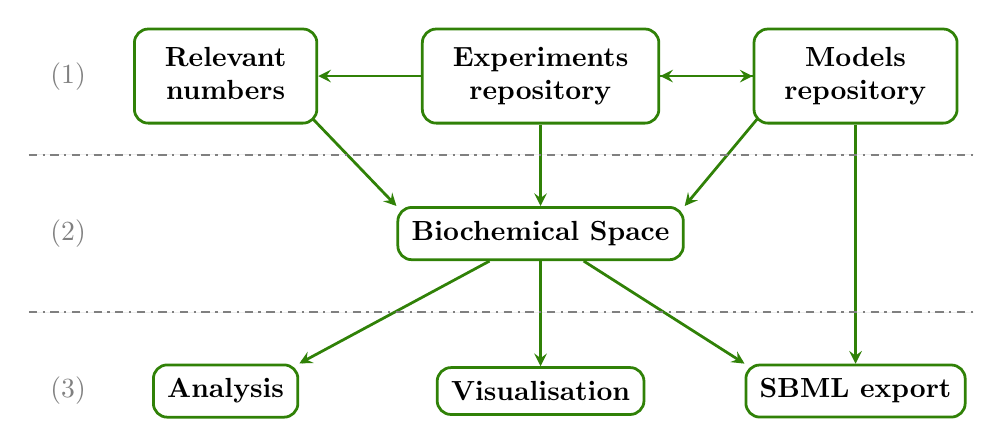
\begin{tikzpicture}[scale=1, transform shape, boxed/.style={rectangle, draw, line width=1pt, inner sep=5pt, rounded corners=5pt}]

% nodes ------------------------------------------------------------------------
\node [draw=mydarkgreen, boxed] (numbers) at (-2, 28) {\begin{tabular}{c}
                              \textbf{Relevant} \\
                              \textbf{numbers}
                          \end{tabular}};
\node [draw=mydarkgreen, boxed] (exper) at (2, 28) {\begin{tabular}{c}
                              \textbf{Experiments} \\
                              \textbf{repository}
                          \end{tabular}};
\node [draw=mydarkgreen, boxed] (models) at (6, 28) {\begin{tabular}{c}
                              \textbf{Models} \\
                              \textbf{repository}
                          \end{tabular}};

\node [draw=mydarkgreen, boxed] (bcs) at (2,26) {\textbf{Biochemical Space}};

\node [draw=mydarkgreen, boxed] (visual) at (2,24) {\textbf{Visualisation}};
\node [draw=mydarkgreen, boxed] (sbml) at (6,24) {\textbf{SBML export}};
\node [draw=mydarkgreen, boxed] (analysis) at (-2, 24) {\textbf{Analysis}};

\node [color=graybright] (1) at (-4, 28) {(1)};
\node [color=graybright] (2) at (-4, 26) {(2)};
\node [color=graybright] (3) at (-4, 24) {(3)};

% arrows ------------------------------------------------------------------------
\draw[myarrow, draw=mydarkgreen, fill=mydarkgreen, shorten <=-3pt, shorten >=1pt, line width=1pt] (numbers.south east) to (bcs.north west);
\draw[myarrow, draw=mydarkgreen, fill=mydarkgreen, shorten >=1pt, line width=1pt] (exper) to (bcs);
\draw[myarrow, draw=mydarkgreen, fill=mydarkgreen, shorten <=-3pt, shorten >=1pt, line width=1pt] (models.south west) to (bcs.north east);

\draw[myarrow, draw=mydarkgreen, fill=mydarkgreen, shorten >=1pt, line width=1pt] (models) to (exper);
\draw[myarrow, draw=mydarkgreen, fill=mydarkgreen, shorten >=1pt, line width=1pt] (exper) to (models);
\draw[myarrow, draw=mydarkgreen, fill=mydarkgreen, shorten >=1pt, line width=1pt] (exper) to (numbers);

\draw[myarrow, draw=mydarkgreen, fill=mydarkgreen, shorten >=1pt, line width=1pt] (bcs) to (visual);
\draw[myarrow, draw=mydarkgreen, fill=mydarkgreen, shorten >=1pt, line width=1pt] (bcs) to (analysis.north east);
\draw[myarrow, draw=mydarkgreen, fill=mydarkgreen, shorten >=1pt, line width=1pt] (bcs) to (sbml.north west);

\draw[myarrow, draw=mydarkgreen, fill=mydarkgreen, shorten >=1pt, line width=1pt] (models) to (sbml);

\draw[thick, dash dot, draw=graybright, fill=graybright] (-4.5, 27) -- (7.5, 27);
\draw[thick, dash dot, draw=graybright, fill=graybright] (-4.5, 25) -- (7.5, 25);
\end{tikzpicture}
\end{center}
\caption{An overview of Comprehensive Modeling Platform. It is composed by three layers: (1) input to the platform, all the relevant data; (2) Biochemical Space as a intermediate format for the data; (3) output of the platform, results of analyses and visualisations.}\label{cmp_overview}
\end{figure}

\subsection{Biochemical Space}
\label{bcs_general}

The platform consists of several dedicated modules (Fig.~\ref{cmp_overview}), all connected to a central module -- \emph{Biochemical Space} (BCS)~\cite{BCS} -- what is the backbone of the platform. BCS provides formal description and annotation of the biological system and it is based on the hierarchy of selected biological processes. It is accompanied with schemas representing relevant biological processes in the context of the modelled system. For each process, there are presented relevant models, chemical entities, and rules. Presentation of every process includes detailed information and links to relevant internal and external sources.

BCS provides a well-described biological background for mathematical models of processes taking place in specific organism. Complete BCS provides a connection between existing ontologies and partial mathematical models. BCS offers a human readable format which can be easily edited in a dedicated editor and visualised within the platform. First part of a BCS is represented by a set of \emph{entities}, while the second part contains \emph{rules}.

When building the BCS, emphasis is put on well-defined and complete annotations. Therefore, links to relevant ontologies must be specified for each entity and rule. Unique IDs provided by ontologies can help to automatically detect duplicities. IDs are also used to create hypertext links to related ontologies on the web, thus providing a one part of the already mentioned connection between ontologies and models. At this moment, links to KEGG~\cite{Kanehisa04012016}, ChEBI~\cite{ChEBI}, CyanoBase~\cite{CyanoBase}, and other databases are supported (example of usage is in Figure~\ref{database_links}). A single entity or a rule can have multiple links to several external databases. An example is presence of a particular entity in ChEBI as well as in KEGG.

\begin{figure}[!h]
\begin{center}
\framebox{
{\footnotesize
\begin{tabular}{ l | l }
 DESCRIPTION: & Protein involved in hydrolysis of N-acetylated amino acids\\
 LINKS: & KEGG::ec3.5.1.14, CBS::slr1653, CBS::sll0100\\
 NOTES: & ChEBI link is missing
\end{tabular}}
}
\end{center}
\caption{Description, links, and notes information for an entity.}\label{database_links}
\end{figure}

The fact that most attributes in entity and rule definitions are tightly coupled with information from linked ontologies is the reason why we have started with describing annotation attributes. In the first place, one of these attributes is \emph{name}, which is taken from ontologies or follows the standard naming conventions. ID of every entity is fixed by the consortium. KEGG ID, ChEBI ID or internal ID is used if no reasonable ID is available. IDs of rules are internal.

\begin{figure}[!h]
\begin{center}
\framebox{
{\footnotesize
\begin{tabular}{ l | l }
 ENTITY ID: & HCO3\\
 STATES: & \{-, +\}\\
 LOCATIONS: & cyt, liq\\
 COMPOSITION:\\
 ENTITY NAME: & hydrogencarbonate\\
 CLASSIFICATION: & small molecule\\
 DESCRIPTION: & Plays major role in carbon concentrating\\
 & mechanism (CCM).\\
 LINKS: & CHEBI::17544\\
 ORGANISM: & Synechococcus elongatus PCC 7942\\
\end{tabular}}
}
\end{center}
\caption{Complete information given for an atomic entity.}\label{entity_example}
\end{figure}

An entity in our interpretation is a bounded space (a so-called \emph{compartment}) or a structural part of a specific organism (for an example see Figure~\ref{entity_example}). BCS covers a hierarchy of \emph{entities} (or \emph{agents}) ranging from small molecules (\emph{atomic entity}) through composite structures (\emph{structure entity}) to large complex molecules (\emph{complex entity}). Our goal is to make BCS as simple as possible. In existing ontologies, entities residing in several different states (oxidised, reduced, etc.) are usually treated as separate entities, thus causing the total number of entities to be enormous. To reduce this complexity, the concept of \emph{states} is defined in BCS. They allow to define allowed set of states, in which an atomic entity can occur.

BCS extends the traditional concept of compartmentalisation with a hierarchy at the level of entities. A particular entity can reside in several different compartments. Additionally, \emph{classification} specifies the type of an entity in a sense of functional or structural characterisation.

An atomic entity can be a part of a structurally more complex entity. We consider two kinds of composite entities: structure (Figure~\ref{structure_example}) and complex entities. Structure entity represents partially specified composite species, for example a photosystem complex partially specified with prosthetic groups of interest. Complex entity represents fully specified composite species, for example, a homodimer of KaiC protein.

\begin{figure}[!h]
\begin{center}
\framebox{
{\footnotesize
\begin{tabular}{ l | l }
 ENTITY ID: & KaiC\\
 STATES:\\
 LOCATIONS: & cyt\\
 COMPOSITION: & S $|$ T\\
 ENTITY NAME: & circadian clock protein kinase KaiC\\
 CLASSIFICATION: & enzyme\\
 DESCRIPTION: & Monomer component representing a core component\\
 & of the circadian clock system.\\
 LINKS: & uniprot::Q79PF4, cyanobase::Synpcc7942\_1216\\
 ORGANISM: & Synechococcus elongatus PCC 7942
\end{tabular}}
}
\end{center}
\caption{Complete information given for a structure entity.}\label{structure_example}
\end{figure}

Rules are specified by \emph{rule equations} enriched with additional annotation information. When defining a rule equation, identifiers of substrates and products are used to make the notation of the rules compact. Every entity appearing in a \emph{rule equation} has to be followed by the localisation operator associating it with a particular compartment. This is important especially for rules that act on both sides of a membrane. That way, a rule is always precisely localised in or between compartments. A natural stoichiometric coefficient can be placed before any entity in a rule equation. Irreversible and reversible rules are distinguished by the operators `$\Rightarrow$', `$\Leftrightarrow$'. The `$+$' symbol is used as a separator between individual substrates and individual products. A rule can also have an assigned classification. Rule classification assigns a list of higher level biophysical processes in which the rule is involved. For an example, see Figure~\ref{rule_example}.

\begin{figure}[!h]
\begin{center}
\framebox{
{\footnotesize
\begin{tabular}{ l | l }
 RULE ID: & NADPH oxid.\\
 RULE EQUATION: & $NADPH :: cyt + 5 h\{$\arc$\} :: cyt + pq :: cym \Rightarrow$\\
 & $\Rightarrow NADP\{$\arc$\} :: cyt + 4 h\{$\arc$\} :: pps + pqh2 :: cym$\\
 MODIFIER: & NDH1\\
 RULE NAME: & plastoquinone reduction in the cytoplasmic membrane\\
 CLASSIFICATION: & reduction, oxidation\\
 DESCRIPTION: & Oxidation of NADPH and reduction of plastoquinone\\
 & in the cytoplasmic membrane.\\
\end{tabular}}
}
\end{center}
\caption{Complete information for a rule.}\label{rule_example}
\end{figure}

In some cases, emphasis on a detailed description leads to very complex BCS models. Abstraction of some processes is needed to keep BCS models as simple as possible. To this end, rules expressing enzymatic reactions are considered in a simplified form. In fact, there should be at least two different rules describing an enzymatic reaction (one for a substrate binding and another for a catalytic step). Instead, since an enzyme is not affected during the reaction, it is affiliated to the rule as a \emph{modifier}. However, it is difficult to define precise meaning of a modifier in this case. We rather treat the modifier attribute informally as an entity \textit{which has to be present} for the rule to be enabled. The exact reaction mechanism of an enzyme is not always clear and therefore it is abstracted out.

\begin{figure}[!h]
\begin{center}
\framebox{
{\footnotesize
\begin{tabular}{ l | l }
 RULE ID: & FGFR2 phosph.\\
 RULE EQUATION: & $Thr\{u\}::FGF::FGFR2::cyt \Leftrightarrow $\\
 & $\Leftrightarrow Thr\{p\}::FGF::FGFR2::cyt$\\
 MODIFIER: & NDH1\\
 RULE NAME: & FGFR2 threonine residue (de)phosphorylation\\
 CLASSIFICATION: & phosphorylation, dephosphorylation\\
 DESCRIPTION: & FGF enzyme is phosphorylated on threonine residue\\
 & in FGFR2 complex.\\
\end{tabular}}
}
\end{center}
\caption{A rule employing structure entity state change. A Threonine ($Thr$) amino acid residue of a $FGF$ protein inside a $FGFR2$ complex can change its state from unphosphorylated ($u$) to phosphorylated ($p$).}
\end{figure}

Higher abstraction comes into account when several electrons play `musical chairs' inside protein complexes. The issue is that parts of processing protein complex can have different unstable states during a short period of time. When one tries to define all rules among these proteins, combinatorial explosion of the number of states of the complex arises. Not all of these combinations are biologically correct. Even when excluding biologically inadmissible cases, the number of states is still enormous. For the purpose of BCS, we introduce a solution -- we treat a protein complex as a structure entity on which structurally simpler atomic entities change their states (not necessarily proteins) and we abstract from background processes.

When describing particular process or object we can go almost infinitely deeper into details. Even if the depth is not infinite, it is deep enough to lead into state when the description is larger than object itself. Imagine that you want to describe a molecule as position of each atom. You definitely need more space to store such information than the molecule itself occupies.

When creating a BCS, we choose a level of details which we do not exceed. This ensures the size of BCS will not exponentially increase with additional details. The problem can occur when we try to map a model which uses more detailed description of the system than BCS does. However, we simply allow relating multiple model objects to BCS objects and \emph{vice versa}. For example, multiple model reactions might be mapped on one BCS rule denoting the fact the process represented by the rule can be described in more details by the reactions. On the other hand, model might neglect some details. Then for example, a reaction can be mapped on multiple rules with similar meaning than in previous case.

Since CMP allows export of models in SBML format, we employ resolvable identifier links~\cite{juty2011identifiers}. These links are included in generated SBML file and point to appropriate rules and entities in BCS.

\subsection{Model Repository}
\label{model}

Model repository is a collection of implemented mathematical models describing particular parts of biological processes. Every model is represented as a set of ordinary differential equations generated from the model reaction network. Models are integrated within BCS. In particular, each model component should be related to some BCS entity and each model reaction should be related to some BCS rule. The model is associated with some parameter value sets (data sets) that enable simulation in a particular biologically-relevant scenarios. Additionally, several basic non-parameter-specific static analysis techniques based on model stoichiometry are also provided.

An implemented model then includes complete biological annotation of all components and reactions that is provided by mapping to BCS. This might help to find connections and overlaps among models. Further, implemented model can be exported to SBML.

\subsection{Experiments Repository}

Experiments repository is a module for storage and presentation of time-series data from wet-lab experiments. Every experiment is well-grounded by precise description (device, medium, organism, etc.) and appropriate annotations. Experiments are structured -- several time series data can be attached to a single experiment. Every time series targets a specific list of measured substances together with time stamps of the individual measurements. Data can be imported and exported in simple text formats. Time series are visualised in a chart.	

\chapter{Problem formulation}
\label{problem_formulation}

Biochemical Space as described in Section~\ref{bcs_general} can grow to quite a huge size. It means keep it consistent on an informal level is almost impossible. It is necessary to be able to detect inconsistency with automatic tools and enable further analysis of the space.

In our last paper~\cite{Ded201627}, we defined Biochemical Space Language (BCSL) such that syntax was defined independently, but semantics were defined via translating to Kappa language~\cite{kappa_formal}. First of all, we wanted to keep the language as concise as is possible. Rule-based approach was the best hit, because it is capable to capture required details for biological systems while keeping the description concise. It was supposed to be human-readable, which in this context means easy to read, write and maintain by humans even from other disciplines than computer science. However, there are many rule-based languages and each of them is slightly different in syntactic and semantic level and also on level of abstraction. After a research (Section~\ref{rule_based_languages}), we have evaluated all existing languages as not suitable for our purposes. The closest representation to the desired one was Kappa language (Section~\ref{kappa}). That is the reason why in first iteration we have chosen translation to Kappa for definition of semantics.

However, we realised this approach is not very beneficial since we are not fully using the expressive power of our language this way. The problem is Kappa operates purely on expressions. We want to promote our language to a higher level when it operates on objects in multisets. By translating to Kappa we loose such abstraction. 

In the previous version of language development, both definition and implementation were made via translation to Kappa. It particularly means there was defined a translation function, which was able to convert BCSL expressions to Kappa expressions. The huge advantage was that the conversion was quite straightforward and this way we could apply all analyses Kappa language has.

The indirect approach had several disadvantages. First of all, Kappa has only one type of agent (no hierarchy). It follows all additional information encoded in different agent types are lost during the conversion. This particularly means atomic agents had to be considered as binding sites and structure agents as Kappa agents. But it was not always suitable, especially when atomic agents had independent role in a rule. Complex treatment in Kappa requires explicit bonds between individual agents. Therefore, when translating our multiset-based complex agent to Kappa complex, we need to choose one of many possible isomorphisms (Figure~\ref{abstraction_comparision}, the biology corresponds to Kappa approach). Multiple default options are available, such as circular layout, linear layout etc. But it was not possible to express fact that order does not matter.

\begin{figure}[!h]
\begin{center}
  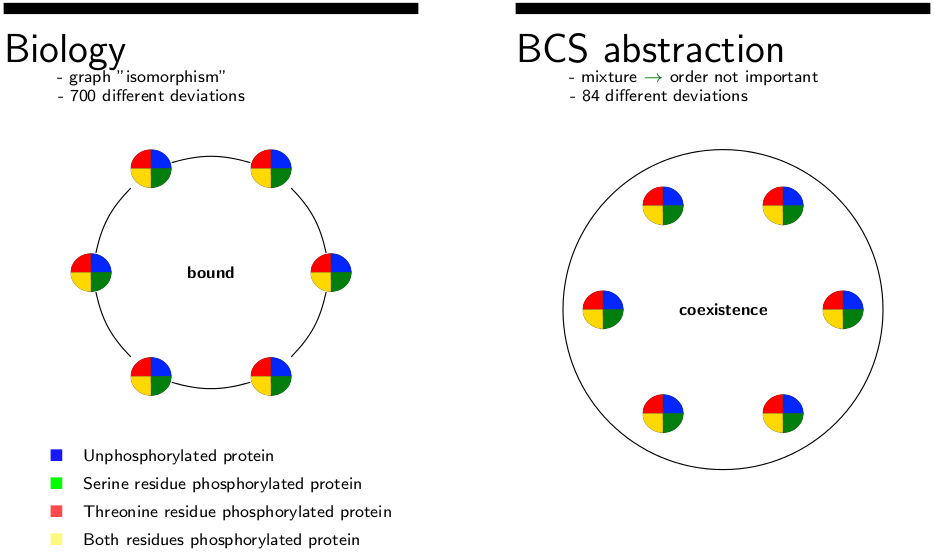
\includegraphics[scale=0.35]{pics/abstraction}
\end{center}
\caption{Comparison of a complex in biology (on the left) to abstraction used in BCS (on the right). In biology, all possible graph isomorphisms must be considered which results from combinatorial options how edges can be placed to create a connected graph~\cite{Chartrand1985}. In BCS we neglect such details and see created structure only in sense of coexistence (a multiset), which significantly reduces number of possible deviations.}\label{abstraction_comparision}
\end{figure}

From the implementation point of view, executing models was delayed by conversion to Kappa and then calling Kappa core to execute its semantics. Moreover, Kappa uses network-free simulator, which is very efficient for small models, because the rules are executed directly. Each rule is being matched on current state and then matched objects are replaced according the rule. The problem is when model is more complex. The number of rules does not cause significant change, however number of different interacting agents does. Once there are many agents, the time of one \emph{match \& replace} step rises dramatically. Compared to indirect methods when first reaction network is enumerated, the initial step can be resources consuming, but then rule application itself is fast regardless number of agents.

For the reasons mentioned above we decided to redefine the BCSL language itself. Particularly, the syntax definition had to be refined in order to make the usability more clear. From semantic point of view, we needed a straightforward definition which would have practical use in implementation. With experiences from previous iteration, it showed that direct rule-based semantics where not very efficient mechanism to be is used. For that reason, we have chosen an indirect definition via translation to reactions -- \emph{practical} definition (Section~\ref{formal_definition}). The practical part means that this approach can be efficiently used in implementation.

In section~\ref{bcs_general}, we have motivated the level of abstraction we need to use in BCS. To achieve that, we decided to neglect structural details, i.e. we do not employ binding approach. We consider binding as too low level of details. Instead, we improve definition of interacting agents to higher level, when an agent might expresses some kind of structural description (Figure~\ref{abstraction_comparision}). This way we avoid complicated creation of complexes and reduce complicated syntax.

Also, we determine two types of complexes. None of them is literally a complex, we rather see it as a coexistence. It allows us to express even other types of interaction. We also determine whether the expresses complex is complete, i.e. the enumerated subparts are all which form the complex. The other type of complex expresses the fact that subparts play an important role in the complex, but there are more parts which we do not model, but this fact is important for semantics of the model.

\chapter{Formal definition}
\label{formal_definition}

In this chapter, we define Biochemical Space Language formally. First, we define all the required objects, then we define syntax of the language and semantics of the BCSL models.

The defined semantics is indirect, i.e. we don't give semantic sense to rules themselves, rather provide a procedure how to generate reactions from the rules and give semantics to them.

For better readability, we provide examples of syntax for most important object during their definition. However, the formal definition of syntax and the relation to the objects will be given later.

\section{Formal preliminaries}

Before we proceed, we recall some basic notations and provide all necessary definition in order to build formal definition for the language.

%We define projection $\pi_i$ to enable iterating through multidimensional structures.

\begin{definition}{Projection}
Projection $\pi_i : X^n \rightarrow X $ is defined as follows:

\begin{center}
$ \pi_i(x_1, \ldots, x_n) = x_i $
\end{center}

for some $i, n \in \mathbb{N}$ and $i \leq n$.
\end{definition}

%Next, we need to define tuples concatenation, since we work with them quite often want to make sure this operation is clear.

\begin{definition}{Tuples concatenation}

Let $X = (x_1, \ldots, x_n), Y = (y_1, \ldots, y_m)$ be two tuples for some $n, m \in \mathbb{N}$. Concatenation of two tuples, written $X \mdoubleplus Y$, is defined as:

\begin{center}
$X \mdoubleplus Y = (x_1, \ldots, x_n, y_1, \ldots, y_m)$.
\end{center}
\end{definition}

%Then, we can generalise concatenation operation to multiple tuples.

\begin{definition}{Sum of concatenations}

Let $T = (T_1, T_2, \ldots, T_n)$ be sequence of tuples. Concatenation of sequence of tuples $\mdoubleplus_{i=1}^n T_i$ is defined as:

\begin{center}
$\mdoubleplus_{i=1}^n T_i = T_1 \mdoubleplus T_2 \mdoubleplus \ldots \mdoubleplus T_n $
\end{center}
\end{definition}

%A non-crossing partition of $S$ is a partition in which no two blocks "cross" each other.

\begin{definition}{Non-crossing partition}
A partition $\mathcal{P} = B_1/B_2/\ldots/B_k$ of $S = [1,\ldots,n]$ is non-crossing if  whenever a quadruple of elements $1 \leq a < b < c < d \leq n$ satisfies $a, c \in B_i$ and $b, d \in B_j$ for some $1 \leq i, j \leq k$, then in fact $i = j$; thus, the blocks do not cross.
\end{definition}

%We also need to use permutations product. For this purpose, we use common notion $\sigma$.

\begin{notation}
Let $\vv{v} = (x_1, \ldots, x_n)$ be a vector. By $\sigma(\vv{v})$ we denote set of all possible permutations with length $n$ of the vector $\vv{v}$.
\end{notation}

\begin{definition}{Labelled transition system}\label{lts}
\textit{Labelled transition system} (LTS) $\mathcal{L}$ is a quadruple $(S, A, \Delta, s_0)$ where:

\begin{itemize}
  \item $S$ is a (potentially infinite) set of states (solutions),
  \item $A$ is a set of labels (reactions),
  \item $\Delta \subseteq S \times A \times S$ is a transition relation (the map-apply action),
  \item $s_0 \in S$ is the initial state (initial solution).
\end{itemize}
\end{definition}

\section{Objects definition}

Let $\mathcal{N}_{A},~\mathcal{N}_{T},~\mathcal{N}_{\delta},~\mathcal{N}_{c}$ be mutually exclusive finite sets of atomic names, structure names, states, and compartments, respectively. Moreover, $\varepsilon$ is reserved symbol and does not belong to any of these sets.

\begin{definition}{Signature}
Atomic signature $\Sigma_{\mathtt{A}} \subseteq \mathcal{N}_{A} \times 2^{\mathcal{N}_{\delta}}$ associates atomic names with set of state names. 

Structure signature $\Sigma_{\mathtt{T}} \subseteq \mathcal{N}_{T} \times 2^{\mathcal{N}_{A}}$ associates structure names with set of atomic names. 
\end{definition}

Signatures define for an atomic name allowed set of states and for a structure name allowed set of atomic names. The deeper meaning will be revealed after next part of definitions.

\begin{example}{Signature}\label{example:signature}
\begin{itemize}
\item An atomic signature $(S, \{u, p\})$, $(Q, \{a, i\})$
\item A structure signature $(KaiC, \{S, Q\})$
\end{itemize}
\end{example}

\begin{definition}{Atomic agent}
Atomic agent $\mathtt{A}$ is a pair $(\eta, \delta)$ where $\eta \in \mathcal{N}_{A}$ is a name and \\ $\delta~\in~\mathcal{N}_{\delta} \cup \{ \varepsilon \}$ is a state.
\end{definition}

Atomic agents are the simplest objects used for describing biological entities. An atomic signature with the same name as the atomic agent defines all allowed states for it (with additional $\varepsilon$ state).

\begin{notation}
Let $\mathtt{A}$ be an atomic agent. We denote by $\eta(\mathtt{A})$ its name and by $\delta(\mathtt{A})$ its state.
\end{notation}

\begin{definition}{Equivalence of atomic agents}
Let $\mathtt{A},~ \mathtt{A}'$ be atomic agents. $\mathtt{A}$ is \emph{equivalent} to $\mathtt{A}'$, written $\mathtt{A} \equiv \mathtt{A}'$, iff $\eta(\mathtt{A}) \equiv \eta(\mathtt{A}') \wedge \delta(\mathtt{A}) \equiv \delta(\mathtt{A}')$.
\end{definition}

\begin{notation}
Let $\mathds{A}$ be universe of all possible atomic agents.
\end{notation}

Universe $\mathds{A}$ represents all atomic agents which can be formed according to defined sets of atomic names and states.

Atomic agents are usually used to express small biological entities which can change their state, for example amino acids, small inorganic molecules etc.

\begin{example}{Atomic agents}\label{example:atomic}

\begin{itemize}
\item An atomic agent $\mathtt{A}_1 = (S, u)$
\begin{itemize}
	\item written as $S\{u\}$.
\end{itemize}
\item An atomic agent $\mathtt{A}_2 = (Q, \varepsilon)$
\begin{itemize}
	\item written as $Q\{\varepsilon\}$.
\end{itemize}
\end{itemize}
\end{example}

Please note state $\varepsilon$ does not mean the agent is in \emph{none} state, but rather the state is unknown or not important.

\begin{definition}{Structure agent}
Structure agent $\mathtt{T}$ is a pair $(\eta, \gamma)$ where $\eta \in \mathcal{N}_{T}$ is a name and $\gamma \subseteq \mathds{A}$ is a set of atomic agents called partial composition.
\end{definition}

A structure agent represents a biochemical object that is composed from several known atomic agents while we know that a composition is abstract and not necessarily complete. To incorporate such an abstraction of biological structures into our language, a structure agent is defined to be labeled with a unique name and it is constructed only from atomic agents considered in the same physical compartment.

\begin{notation}
Let $\mathtt{T}$ be a structure agent. We denote by $\eta(\mathtt{T})$ its name and by $\gamma(\mathtt{A})$ its partial composition.
\end{notation}

\begin{definition}{Equivalence of structure agents}
Let $\mathtt{T}, \mathtt{T}'$ be structure agents. $\mathtt{T}$ is \emph{equivalent} to $\mathtt{T}'$, written $\mathtt{T} \equiv \mathtt{T}'$, iff $\eta(\mathtt{T}) \equiv \eta(\mathtt{T}') \wedge \gamma(\mathtt{T}) \equiv \gamma(\mathtt{T'})$.

%\forall \mathtt{A} \in \gamma(\mathtt{T}) ~\exists \mathtt{A}' \in \gamma(\mathtt{T}') : \mathtt{A} \equiv \mathtt{A}' \wedge \forall \mathtt{A}' \in \gamma(\mathtt{T}') ~\exists \mathtt{A} \in \gamma(\mathtt{T}) : \mathtt{A}' \equiv \mathtt{A}$.
\end{definition}

The key construct of a structure agent is \emph{partial composition} defined as a list of atomic agents which are considered to be relevant parts of the structure agent. We allow this list to be empty with the meaning of a biological structure for which we do not know its composition.

\begin{notation}
Let $\mathds{T}$ be universe of all possible structure agents.
\end{notation}

Universe $\mathds{T}$ represents all structure agents which can be formed according to defined sets of atomic names, structure names, and states.

A typical example of a structure agent is a protein where the atomic agents are individual amino acids that are of interest in the particular setting.

\begin{example}{Structure agent}\label{example:structure}
\begin{itemize}
\item A structure agent $\mathtt{T}_1 = (K, \textcolor{red}{\{}(S, p), (Q, i)\textcolor{red}{\}})$
\begin{itemize}
	\item written as $K(S\{p\}, Q\{i\})$.
\end{itemize}
\item A structure agent $\mathtt{T}_2 = (K, \textcolor{red}{\{}(Q, a)\textcolor{red}{\}})$
\begin{itemize}
	\item written as $K(Q\{A\})$.
\end{itemize}
\end{itemize}
\end{example}

\begin{definition}{Complex agent}
Complex agent $\mathtt{X}$ is a pair $(\mu, \mathtt{com})$ where $\mu \in (\mathds{A} \cup \mathds{T})^n$ is a sequence of agents, $\mathtt{com} \in \mathcal{N}_{c}$ is a compartment, and $n \in \mathbb{N}$.
\end{definition}

A complex agent represents a non-trivial composite biochemical object that is inductively constructed from already known biological objects. In common rule-based languages this is typically defined by introducing bonds between individual biochemical objects. In BCSL we abstract from detailed specification of bonds and we rather assume a complex as a coexistence of certain objects in a particular group. Moreover, a complex agent resides in a compartment which gives it a space position. 

\begin{definition}{Equivalence of complex agents}\label{rule_equiv}
Let $\mathtt{X}, \mathtt{X}'$ be complexes. $\mathtt{X}$ is \emph{equivalent} to $\mathtt{X}'$, written $\mathtt{X} \equiv \mathtt{X}'$, iff $|\mu(\mathtt{X})| \equiv |\mu(\mathtt{X'})| \wedge \exists \mu' \in \sigma(\mu(\mathtt{X}'))$ such that $\forall i~\in~[1,~n]: \pi_i(\mu(\mathtt{X})) \equiv \pi_i(\mu')$.
\end{definition}

The key element of a complex agent is \emph{sequence} describing inductively constructed coexistence expressions from existing agents. In contrast to partial composition in structure agent, we allow replication at the level of sequence (an agent of a certain name can appear more than once in a sequence).

\begin{notation}
Let $\mathds{X}$ be universe of all possible complex agents. Additionally, we denote $\mathds{U}~=~\mathds{A}~\cup~\mathds{T}~\cup~\mathds{X}$ as universe of all possible agents.
\end{notation}

\begin{example}{Complex}\label{example:complex}

\begin{itemize}
\item A complex $\mathtt{X} = (\textcolor{green}{(}(K, \textcolor{red}{\{}(S, p), (Q, i)\textcolor{red}{\}}), (S, p)\textcolor{green}{)}, cytosol)$
\begin{itemize}
	\item written as $K(S\{p\}, Q\{i\}).S\{p\}::cytosol$
\end{itemize}
\end{itemize}
\end{example}

The complex agents have very important role in the language. It means, an atomic or structure agent cannot exist on its own, it must be encapsulated in a complex (which might have only one item in its sequence). This guarantees each atomic and structure agent has indirectly given space location -- the compartment.

\begin{definition}{Rule}
\label{rule_definition}

Rule $\mathtt{R}$ is a quintuple $(\chi, \omega, \iota, \varphi, \psi)$ where:

\begin{itemize}
\item $\chi \in \mathds{X}^n$ is a sequence of complexes,
\item $\omega \in (\mathds{A} \cup \mathds{T})^m$ is a sequence of atomic and structure agents,
\item $\iota \in \{ 1, \ldots, n \}$ is an index determining start of right-hand-side,
\item $\varphi \in \mathbb{N}^m$ is an index map between $\omega$ and $\chi$,
\item $\psi \in ((\{-\} \cup \mathbb{N})^2)^n$ is an index map between agents from left and right-hand side.
\end{itemize}

where $n, m \in \mathbb{N}$.
\end{definition}

The rule is quite a complicated structure. The reason is the practical definition of semantics which can be seen in following sections. Also, it is necessary to capture relationship between left and right-hand side of the rule. This is done by enumerating all atomic and structure agents in $\omega$ and consequently creating index map between the agents in $\psi$. Another index map $\varphi$ serves for relating agents from $\omega$ back to original sequence of complexes $\chi$. Finally, by index $\iota$ we determine the end of left-hand side of the rule.

\begin{notation}
Let $\mathds{R}$ be universe of all possible rules.
\end{notation}

\begin{example}{Rule}\label{example:rule}

\begin{itemize}
\item 
$\chi = \begin{bmatrix}
(\textcolor{green}{(} (K, \textcolor{red}{\{}(S, u)\textcolor{red}{\}}), (B, \textcolor{red}{\emptyset}) \textcolor{green}{)}, cyt),\\

(\textcolor{green}{(} (C, \textcolor{red}{\emptyset}), (D, i) \textcolor{green}{)}, cyt),\\

(\textcolor{green}{(} (A, \varepsilon) \textcolor{green}{)}, cyt),\\

(\textcolor{green}{(} (K, \textcolor{red}{\{}(S, p)\textcolor{red}{\}}), (B, \textcolor{red}{\emptyset}), (C, \textcolor{red}{\emptyset}) \textcolor{green}{)}, cyt),\\

(\textcolor{green}{(} (D, a), (A, \varepsilon) \textcolor{green}{)}, cyt),\\

(\textcolor{green}{(} (H, u) \textcolor{green}{)}, cyt)  
\end{bmatrix}$

\item $\omega = \begin{bmatrix}
(K, \textcolor{red}{\{}(S, u)\textcolor{red}{\}}), (B, \textcolor{red}{\emptyset}), (C, \textcolor{red}{\emptyset}), \\
(D, i), (A, \varepsilon), (K, \textcolor{red}{\{}(S, p)\textcolor{red}{\}}), \\
(B, \textcolor{red}{\emptyset}), (C, \textcolor{red}{\emptyset}), (D, a), (A, \varepsilon), (H, u)
\end{bmatrix}$

\item $\iota = 3$
\item $\varphi = (2,4,5,8,10,11)$
\item $\psi = [ (1,6) ; (2,7) ; (3,8) ; (4,9) ; (5,10) ; (-,11) ] $
\end{itemize}
 written as:

\begin{center}
\hspace*{-2cm}{\small $K(S\{u\}).B(\varnothing)::cyt + C(\varnothing).D\{i\}::cyt + A\{\varepsilon\}::cyt \Rightarrow$ 

$\Rightarrow K(S\{p\}).B(\varnothing).C(\varnothing)::cyt + D\{a\}.A\{\varepsilon\}::cyt + H\{u\}::cyt$}
\end{center}
\end{example}

Not every rule gives a sense. We need to specify, when a rule is \emph{well-formed}, i.e. it gives semantically sense.

\begin{definition}{Well-formed rule}
Let $\mathtt{R}$ be a rule and $i,j \in \mathbb{N}$ natural numbers. We say the rule $\mathtt{R} = (\chi, \omega, \iota, \varphi, \psi)$ is \emph{well-formed} if the following conditions hold:

\begin{enumerate}
	\item \label{cond1} $\exists (i,j) \in \psi: \pi_i(\chi) \not\equiv \pi_j(\chi) $,
	\item \label{cond2} $\forall (i,j) \in \psi: \eta(\pi_i(\omega)) \equiv \eta(\pi_j(\omega))$.
\end{enumerate}

\end{definition}

A rule is well-formed if it does any action. It means, some change has to occur during rule application. This is ensured by condition~(\ref{cond1}), which requires at least one pair of complexes from left and right-hand side of the rule to be different. The second condition~(\ref{cond2}) has to hold on order to guarantee pairs of structure and atomic agents in $\omega$ of the rule have the same name. This condition is crutial for ground form function $\mathcal{G}$ defined in Section~\ref{ground_forms}, where adding context to different agents do not give a sense. 

Please note the conditions for well-formed rules do not apply on those agents which do not have a pair on the other side of the rule.

\begin{definition}{Reaction}

Reaction $\mathtt{r}$ is a pair $(\mathtt{seq}, \iota)$ where:

\begin{itemize}
\item $\mathtt{seq} \in \mathds{X}^n$ is a sequence of complexes,
\item $\iota \in \{ 1, \ldots, n \}$ is an index determining start of right-hand-side
\end{itemize}

where $n, m \in \mathbb{N}$.
\end{definition}

Reaction is similar structure than rule, but much simpler. The reaction is just mediate format for giving semantics to BCSL models and it only holds information about complex contents of the rule.

\begin{notation}
We denote left-hand-side of the reaction $(\pi_1(\mathtt{seq}), \ldots, \pi_{\iota-1}(\mathtt{seq}))$ as $LHS(\mathtt{r})$ and right-hand-side of the reaction $(\pi_\iota(\mathtt{seq}), \ldots, \pi_n(\mathtt{seq}))$ as $RHS(\mathtt{r})$.
\end{notation}

\section{Syntax}
\label{syntax}

In this section, we define grammar for the BCSL. As proposed in Section~\ref{problem_formulation}, the syntax must be simple and readable. It was already defined in~\cite{Ded201627}, here we provide an improved and simplified version of the definition.

\begin{definition}{Grammar}
\begin{center}
\begin{tabular}{ l l }
atomic expression & $\alpha ::= \eta\{s\} ~|~ \eta\{\varepsilon\}$\\
 & $\eta ::= n \in \mathcal{N}_{A}$ \\
 & $s ::= n \in \mathcal{N}_{\delta}$\\
 & \\
structure expression & $\tau ::= \eta(\gamma) ~|~ \eta(\varnothing)$\\
 & $\gamma ::= \alpha_1, \ldots, \alpha_k$ \\
 & $\eta ::= n \in \mathcal{N}_{T}$\\
 & \\
complex expression & $\Gamma ::= \beta_1~.~\ldots~.~\beta_k :: c$\\
 & $\beta_i ::= \alpha ~|~ \tau$\\
 & $c ::= n \in \mathcal{N}_{c}$\\
 & \\
rule expression & $\rho ::= \Gamma_1 + \ldots + \Gamma_n \Rightarrow \Gamma_{n+1} + \ldots + \Gamma_m $
\end{tabular}

\end{center}
where $m,n \in \mathbb{N}_0 \wedge m > n \wedge m + n \neq 0$ and $k \in \mathbb{N}$.
\end{definition}

Examples of syntax can be seen in the previous examples (Example~\ref{example:atomic} to \ref{example:rule}).

\section{BCSL model}
\label{BCSl_model}

When we have defined syntax of BCSL, we can proceed to BCSL model. We always consider initialised model, which means the definition contains an initial state of the system. The definition also contains rule expressions and signatures.

\begin{definition}{BCSL model}
BCSL model $\mathds{M}$ is a quadruple $(\mathcal{R}, \Sigma_\mathtt{A}, \Sigma_\mathtt{T}, \mathtt{init})$ where $\mathcal{R}$ is set of rule expressions, $\Sigma_\mathtt{A}$ is atomic signature, $\Sigma_\mathtt{T}$ is structure signature, and $\mathtt{init}$ is initial multiset of complex expressions $\Gamma$.
\end{definition}

BCSL model is formed by a set of rule expressions $\mathcal{R}$, which define behavior of the model. The initial multiset $\mathtt{init}$ defines the state of the model in the beginning. Atomic signature $\Sigma_\mathtt{A}$ define allowed states for all atomic agents used in the rules. FInally, structure signature $\Sigma_\mathtt{T}$ defines allowed atomic agents for all structure agents used in the rules.

\begin{remark}
At this point it is useful to sum up what is Biochemical Space as described in Section~\ref{bcs_general}. The BCS is formed by a database of entities and rules. These entities are actually a signature, i.e. they predefine a domain on which rules can be defined. Neglecting an initial state (which is not important for entire space), the BCS is actually a BCSL model.
\end{remark}

\section{Additional definitions}

Before we proceed, there are a few necessary definitions. These definitions are required in next section in order to generate reactions from rules.

Reassembly operation is quite a simple action on tuples. Basically, we need to reorganise tuple which has form $((a_1, b_1), (a_2, b_2),\\ \ldots, (a_n, b_n))$ to a tuple of form $(a_1, a_2, \ldots, a_n, b_1, b_2, \ldots,  b_n)$. We define reassembly generally on a set of tuples. 

\begin{definition}{Reassembly}

Let $Y$ be a set of tuples of particular form, where each $y \in Y$ has particular form $((a_1, b_1), (a_2, b_2), \ldots, (a_n, b_n))$. Then:

\begin{center}
$\mathtt{reassembly}(Y) = \{~  x ~|~ y \in Y \wedge x = (\mdoubleplus_{i=1}^{|y|} \pi_1(y_i)) \mdoubleplus (\mdoubleplus_{i=1}^{|y|} \pi_2(y_i)) ~\}$
\end{center}
\end{definition}

We need to define difference of partial compositions of structure agents $\gamma \ominus \gamma'$. This difference is not just set difference, because we are not comparing atomic agents by overall equality, only equality on agent names. This operation is necessary in process of generating reactions from rules, which basically means adding details to partial compositions according to defined signatures.

\begin{definition}{Difference of partial compositions}

Let $\gamma, \gamma'$ be two partial compositions. We define difference of these two sets on names of its atomic agents as follows:

\begin{center}
$\gamma \ominus \gamma' \myeq \{ \eta_\alpha ~|~ \exists \mathtt{A}: (\mathtt{A} \in \gamma \wedge \eta(\mathtt{A}) \equiv \eta_\alpha ) \wedge \not\exists \mathtt{A}': (\mathtt{A}' \in \gamma' \wedge \eta(\mathtt{A}') \equiv \eta_\alpha)\}$
\end{center}
\end{definition}

Similarly as in previous definition, we need to be able to find difference in context of atomic agent names between partial composition and structure signature.

\begin{definition}{Difference of partial composition and structure signature}

Let $\mathtt{T}$ be a structure agent, $\eta$ its name, and $\Sigma_T(\mathtt{T})$ appropriate signature. We define difference of partial composition $\gamma(\mathtt{T})$ and structure signature $\Sigma_T(\mathtt{T})$ as follows:

\begin{center}
$\Sigma_T(\mathtt{\eta}) \ominus \gamma(\mathtt{T}) \myeq \{ \eta_\Sigma ~|~ \eta_\Sigma \in \Sigma_T(\mathtt{\eta}) \wedge \not\exists \mathtt{A}: (\mathtt{A} \in \gamma(\mathtt{T}) \wedge \eta(\mathtt{A}) \equiv \eta_\Sigma)\}$
\end{center}
\end{definition}

\section{Semantic function}
\label{semantic_function}

In the previous sections, we defined BCSL objects and BCSL model. Now, we need to connect them in order to we give semantic meaning to the model $\mathds{M}$. For this purpose, we define semantic function $\mathtt{F}$ (Definition~\ref{semantic_function}). It is defined recursively for a model $\mathds{M}$ according to expression given as an argument.

\begin{definition}{Semantic function}
\label{semantic_function}
\begin{center}
\begin{tabular}{ c c l}
$\mathtt{F} \llbracket ~\eta\{\varepsilon\}~ \rrbracket$ & = & $(\eta, \varepsilon) \in \mathds{A}$\\
 & & \\
$\mathtt{F} \llbracket ~\eta\{s\}~ \rrbracket$ & = & $(\eta, s) \in \mathds{A}$\\
 & & \\
$\mathtt{F} \llbracket ~\eta(\varnothing)~ \rrbracket$ & = & $(\eta, \emptyset) \in \mathds{T}$\\
 & & \\
$\mathtt{F} \llbracket ~\eta(\mathtt{a}_1, \ldots, \mathtt{a}_n)~ \rrbracket$ & = &
$(\eta, \{~ \mathtt{F} \llbracket \mathtt{a}_1 \rrbracket, \ldots, \mathtt{F} \llbracket \mathtt{a}_n \rrbracket ~\}) \in \mathds{T}$\\
 & & \\
$\mathtt{F} \llbracket ~\alpha_1~.~\ldots~.~\alpha_n :: c~ \rrbracket$ & = &
$(~(\mathtt{F} \llbracket ~\alpha_1~ \rrbracket, \ldots, \mathtt{F} \llbracket ~\alpha_n~ \rrbracket), ~c~) \in \mathds{X}$\\
 & & \\
$\mathtt{F} \llbracket ~\Gamma_1 + \ldots + \Gamma_n \Rightarrow \Gamma_{n+1} + \ldots + \Gamma_m~ \rrbracket$ & = &
$(\chi, \omega, \iota, \varphi, \psi) \in \mathds{R}$ :\\
\end{tabular}
\end{center}

\begin{center}
\begin{itemize}
\item $\chi = (\mathtt{F} \llbracket ~\Gamma_1~ \rrbracket, \ldots, \mathtt{F} \llbracket ~\Gamma_n~ \rrbracket, \mathtt{F} \llbracket ~\Gamma_{n+1}~ \rrbracket, \ldots, \mathtt{F} \llbracket ~\Gamma_m~ \rrbracket)$,
\item $\omega = \mdoubleplus_{i=1}^{|\chi|} \mu(\pi_i(\chi))$,
\item $\iota = n$,
\item $\varphi = (J_1, \ldots, J_m): J_k = \sum\limits_{i=1}^{k} | \mu(\pi_i(\chi)) |$,

\item \begin{tabular}{l l}

& \hspace*{-0.3cm} $\{~ (i,j) ~|~ i \in [1, \pi_\iota(\varphi)] \wedge j \in [\pi_\iota(\varphi), |\omega|] \wedge |i-j| \equiv \pi_\iota(\varphi)~\} ~\cup$ \\

\hspace*{-0.3cm}$\psi =$ & \hspace*{-0.3cm} $\{~ (i, -) ~|~ i \in [k, \pi_\iota(\varphi)] \wedge k = |~ \{ \pi_\iota(\varphi) + 1, \ldots, | \alpha | \} ~| ~\} ~\cup$\\

& \hspace*{-0.3cm} $ \{~ (-, j) ~|~ j \in [k, |\alpha|] \wedge k = 2 * \pi_\iota(\varphi) ~\}$
\end{tabular}


\vspace*{0.5cm} where $\psi$ is lexicographically sorted such that $'-' > i$ for every $i \in \mathbb{N}$.

\end{itemize}
\end{center}
\end{definition}

Please note by applying semantic function $\mathtt{F}$ on expressions from Examples~\ref{example:atomic} to \ref{example:rule}, we obtain agents (resp. complex or rule) from appropriate examples. Moreover, semantic function works \emph{only} on BCSL object and rules well-defined by the given grammar (Section~\ref{syntax}).

\section{Ground forms}
\label{ground_forms}

\emph{Ground form} represents appending context to agents according to signature (we assume signature is always available and therefore we omit it in ground from function arguments). Particularly, this process means adding details to partial compositions and adding states of atomic agents according to defined signatures. Since there are typically multiple states allowed for an atomic agent, this processes leads to multiple options how to add a context. This is natural consequence of fact that a rule is an abstract representation of multiple reactions. 

In the Definition~\ref{ground_form}, objects (middle column) of particular type (left column) are transformed to their ground forms by ground form function $\mathcal{G}$ (right column).

In case of single atomic agent $\mathtt{A}$, there are two options -- either the state is $\varepsilon$ or the state $\delta$ is given. In first case, we construct a set of all possible atomic agents according to the given atomic signature $\Sigma_A(\eta(\mathtt{A}))$. In the second case, we construct a set containing only the original agent itself.

For a pair of atomic agents $\mathtt{A}, \mathtt{A}'$ we create a set of all possible pairs $(a, a')$ such that these pairs has equal names.

Ground form of a structure agent $\mathtt{T}$ is a set of structure agents $\mathtt{T}'$ such that we \emph{insert} all neglected context information into its partial composition. In other words, we need to determine which atomic agents are missing in the partial composition, which can be obtained from the signature $\Sigma_T(\eta(\mathtt{T}))$. Then we create all possible combinations of inserted atomic agents recursively.

For a pair of structure agents $\mathtt{T}, \mathtt{T}'$ we expand both partial compositions recursively such that the expanded parts are equal, i.e. we add the same context to both agents. Similarly as in previous cases, we create set of all possibilities of such pairs.

Finally, ground form of a rule $\mathtt{R}$ is a Cartesian product of sets created for each pair of agents by applying ground from function. The pairs are given by order in index map $\psi$.

\begin{definition}{Ground form}
\label{ground_form}
{\small
\begin{center}
\begin{tabular}{ c c c }
\textbf{Type} & \textbf{Notation} & \textbf{Ground form} \\
 & & \\
\hline
 & & \\
$\mathds{A}$ & $\mathcal{G}(\eta, \varepsilon)$ & $\{~ (\eta, \delta) ~|~ \delta \in \Sigma_A(\eta) ~\}$\\
 & $\mathcal{G}(\eta, \delta)$ & $\{~(\eta, \delta) ~\}$\\
 & & \\
  \hline
 & & \\
 $\mathds{A}^2$ & $\mathcal{G}(\mathtt{A}, \mathtt{A}')$ & $\{~ (a, a') ~|~ a \in \mathcal{G}(\mathtt{A}) \wedge a' \in \mathcal{G}(\mathtt{A}') \wedge \delta(a) \equiv \delta(a') ~\}$\\
 & & \\
 \hline
 & & \\
$\mathds{T}$ & $\mathcal{G}(\eta, \gamma)$ & $
  \Set{ (\eta, \gamma')\ | \begin{array}{l}
  \gamma' \equiv \gamma \cup \gamma_\Sigma \wedge \gamma_\Sigma \subseteq \mathcal{G}(\eta', \varepsilon) ~\wedge \\
  \wedge~ |\gamma_\Sigma| = |\Sigma_T(\eta) \ominus \gamma| \wedge \eta' \in \Sigma_T(\eta) \ominus \gamma \wedge\\
  \wedge~ \forall \widetilde{\eta} \in \Sigma_T(\eta) \ominus \gamma : \widetilde{\eta} \in  \gamma_\Sigma
  \end{array}}$\\
 & & \\
 \hline
 & & \\
$\mathds{T}^2$ & $\mathcal{G}(\mathtt{T}, \mathtt{T}')$ & $
  \Set{ (t, t')\ | \begin{array}{l}
  t \in \mathcal{G}(\mathtt{T}) \wedge t' \in \mathcal{G}(\mathtt{T}') ~\wedge \\
  \wedge~ \gamma(t) \ominus \gamma(\mathtt{T}) \equiv \gamma(t') \ominus \gamma(\mathtt{T}')
  \end{array}}$\\
  & & \\
 \hline
 & & \\
$\mathds{R}$ & $\mathcal{G}(\mathtt{R})$ & $ \displaystyle \prod_{k = 1}^{|\mathcal{G}(\psi)|} \mathcal{G}(\psi)_k $ \\ 
\end{tabular}
\end{center}

\noindent where $\mathcal{G}(\psi)_k = \mathcal{G}(\pi_i(\omega), \pi_j(\omega))$ such that $(i,j) = \pi_k(\psi)$ and $\mathtt{R} = (\chi, \omega, \iota, \varphi, \psi)$. Moreover, $\mathtt{A} = (\eta, \delta)$, $\mathtt{A}' = (\eta', \delta')$, $\mathtt{T} = (\eta, \gamma)$, and $\mathtt{T}' = (\eta', \gamma')$.
}
\end{definition}

\section{Construction of reactions}
\label{Generating reactions}

Given a rule $\mathtt{R}$, we can produce appropriate reactions using ground forms and subsequent application of reassembly operation.

\begin{definition}{Construction of reactions}\label{generate_reactions}
\hspace*{-0.8cm}\begin{tabular}{ r l }
$\mathtt{Reactions}(\mathtt{R}) =$ & $\{~ \mathtt{r}(\mathtt{seq}, \iota) ~|~ y \in \mathtt{reassembly}(\mathcal{G}(\mathtt{R})) ~\}$,\\

where $\mathtt{seq} =$ & $ \big(\mathtt{X}(y(0, \ldots, \pi_0(\varphi) - 1), \mathtt{com}(\pi_0(\chi))),$ \\

& ~~$\mathtt{X}(y(\pi_0(\varphi), \ldots, \pi_1(\varphi) - 1), \mathtt{com}(\pi_1(\chi))), $\\

& ~~\ldots,\\

& ~~$\mathtt{X}(y(\pi_{|\varphi| - 1}(\varphi), \ldots, \pi_{|\varphi|}(\varphi) - 1), \mathtt{com}(\pi_{|\varphi|}(\chi)))\big) $\\

 & ~~and $ \iota \in \mathtt{R}$, $\chi \in \mathtt{R}$, $\varphi \in \mathtt{R}.$\\
\end{tabular}
\end{definition}

\section{Chemical Reaction Networks}

\begin{definition}{Chemical Reaction Model (CRN)}
\label{crn}
Chemical Reaction Model $\mathcal{M}$ is a triple $(\mathfrak{R}, \vv{\nu}, \theta)$ such that $\mathfrak{R} \subseteq \mathbb{Z}^n$ is set of chemical reactions, $\vv{\nu} \in \mathbb{N}_0^n$ is initial vector, and $\theta \in \mathds{X}^n$ is vector of reference complexes for some $n \in \mathbb{N}$.
\end{definition}

Chemical Reaction Model is a simple model, where chemical reactions and initial state are vectors over integers. Moreover, there is a reference vector of complex agents, which servers for identifying underlaying agents behind the integers (according to particular position in vectors).

\begin{notation}\label{nonnegative}
We denote $N(\vv{\nu})$ condition $\forall i \in \vv{\nu}: i \in \mathbb{N}_0$.
\end{notation}

By Notation~\ref{nonnegative} we denote the condition that a vector is formed only by non-negative integers.

\begin{definition}{Chemical reaction application}

Chemical reaction application $\varrho$ is a relation $\varrho \subseteq \mathbb{N}_0^n \times \mathbb{Z}^n \times \mathbb{N}_0^n$ such that 
\begin{center}
$(\vv{\upsilon}, \vv{\mathtt{r}}, \vv{\mathtt{u}}) \in \varrho \myeq \vv{\mathtt{u}} = \vv{\upsilon} + \vv{\mathtt{r}} \wedge N(\vv{\mathtt{u}})$.
\end{center}
\end{definition}

Note some values in chemical reactions might be negative. When applying reaction on state, the resulting state cannot contain any negative values (negative number of entities does not give biological sense). Therefore, application is allowed only if the resulting vector contains non-negative values.

\begin{definition}{CRN semantics}
Let $\mathcal{M}$ be a Chemical Reaction Model. The quantitative semantics are given in terms of a \emph{discrete-states} produced by iterative reaction application on initial vector $\vv{\nu}$ and all consequently created state vectors. This way we obtain an LTS (Definition~\ref{lts}).
\end{definition}

CRN semantics might lead to possibly infinite LTS. This process can be limited by a global bound, which makes sure the produced LTS is finite (Section~\ref{optimal_bound}).

\section{Construction of model}

In previous sections we defined all required constructs to create a Chemical Reaction Model (Definition~\ref{crn}) from a BCSL model. This procedure is necessary in order to allow operational semantics to be applied.

\begin{definition}{Reference vector}\label{reference_vector}

Let $\Theta$ be a set of all possible unique complexes constructed from reactions of model $\mathds{M}$ defined as follows:

$$\Theta = \{~ \mathtt{X} ~|~ \mathtt{X} \in \mathtt{seq}(\mathtt{r}) \wedge \mathtt{r} \in \bigcup_{\mathtt{R} \in \mathcal{R}} \mathtt{Reactions}(\mathtt{R}) ~\} $$

\noindent Then, the \emph{reference vector} $\theta$ is a tuple $X \in \Theta^n$ such that $\forall i,j \leq n : \Theta_i \not\equiv \Theta_j$ and $n~=~|\Theta|$. Note there are $n!$ possibilities how to choose $\theta$, an arbitrary one can be chosen.

\end{definition}

\begin{definition}{Multiset to vector translation}\label{state_to_vector}
Translation of multiset $\mathtt{S} \subseteq \mathds{X}$ to vector is defined as following:
\begin{center}
$\lambda(\mathtt{S}, \theta) = (a_1, a_2, \ldots, a_n)$ such that 
$a_i$ =
  $\begin{cases}
  |\mathtt{S}(\theta_i)| & \ldots~~~~ \theta_i \in \mathtt{S}\\
  0 & \ldots~~~~ \theta_i \not\in \mathtt{S}\\
  \end{cases}
  $
\end{center}
\hspace{15pt} where $n = |\theta|$ and $|\mathtt{S}(\pi_i)|$ is number of occurrences of agent $\pi_i$ in the multiset $\mathtt{S}$.
\end{definition}

Let $\mathds{M} = (\mathcal{R}, \Sigma_\mathtt{A}, \Sigma_\mathtt{T}, \mathtt{init})$ be a BCSL model. In order to construct Chemical Reaction Model $\mathcal{M} = (\mathfrak{R}, \vv{\nu}, \theta)$ from the model $\mathds{M}$, we need to apply the following steps:

\begin{enumerate}
\item generate reactions for all rules $\mathtt{F}(\mathtt{R}) \in \mathcal{R}$ (Definition~\ref{generate_reactions}),
\item construct reference vector $\theta$ (Definition~\ref{reference_vector}),
\item create initial vector $\vv{\nu} = \lambda(\mathtt{S}, \theta)$ from initial multiset $\mathtt{S}$ where $\mathtt{S} = \{ \mathtt{X} ~|~ \mathtt{X} = \mathtt{F}(\Gamma) \wedge \Gamma \in \mathtt{init} \}$ (Definition~\ref{state_to_vector}),
\item construct set of chemical reactions $\mathfrak{R}$ from the set reactions, where individual vector reaction $\vv{r}$ is created from a reaction $\mathtt{r}$ as following:

\begin{center}
$\vv{r} = \lambda(RHS(\mathtt{r}), \theta) - \lambda(LHS(\mathtt{r}), \theta)$
\end{center}

\end{enumerate}

In order to accomplish the process of giving semantics to an BCSL model, it is necessary to note how we revive information which is missing in produced LTS (Definition~\ref{lts}). This procedure is quite straightforward since we have defined reference vector $\theta$. Similarly as we translated multisets of BCSL agents to vectors (Definition~\ref{state_to_vector}), we can apply a reverse procedure, when we build a multiset of agents from a vector according to the reference vector $\theta$.

\section{Syntactic extensions}
\label{syntactic_extensions}

We define several syntactic extensions for better readability of the rules. Note that each rule in an extended form can be always translated to basic form defined above. All rules containing the following extensions must be converted to basic form before semantics can be applied.

For better demonstration we provide a running example, which will go through all syntactic extensions. Please note there is no biological sense of the model, it has only demonstrative purpose.

\begin{runningExample}{The example model $\mathds{M}$}
\label{run1}

\noindent Definition of rules $\mathtt{R}$:
{\footnotesize
\begin{enumerate}
\item $KaiC(S\{u\}, T\{\varepsilon\}).KaiC(S\{\varepsilon\}, T\{\varepsilon\}).KaiC(S\{\varepsilon\}, T\{\varepsilon\})::cyt \Rightarrow $

$\Rightarrow KaiC(S\{p\}, T\{\varepsilon\}).KaiC(S\{\varepsilon\}, T\{\varepsilon\}).KaiC(S\{\varepsilon\}, T\{\varepsilon\})::cyt$

\item $KaiC(S\{u\}, T\{\varepsilon\}).KaiB::cyt \Rightarrow KaiC(S\{p\}, T\{\varepsilon\}).KaiB::cyt$
\item $KaiC(S\{\varepsilon\}, T\{\varepsilon\})::cyt + KaiC(S\{\varepsilon\}, T\{\varepsilon\})::cyt + KaiC(S\{\varepsilon\}, T\{\varepsilon\})::cyt \Rightarrow$ 

$ \Rightarrow KaiC(S\{\varepsilon\}, T\{\varepsilon\}).KaiC(S\{\varepsilon\}, T\{\varepsilon\}).KaiC(S\{\varepsilon\}, T\{\varepsilon\})::cyt$

\item $KaiC(S\{\varepsilon\}, T\{\varepsilon\}).KaiC(S\{\varepsilon\}, T\{\varepsilon\}).KaiC(S\{\varepsilon\}, T\{\varepsilon\})::cyt \Rightarrow $

$\Rightarrow KaiC(S\{\varepsilon\}, T\{\varepsilon\})::cyt + KaiC(S\{\varepsilon\}, T\{\varepsilon\})::cyt + KaiC(S\{\varepsilon\}, T\{\varepsilon\})::cyt$
\end{enumerate}
}

\noindent Definition of $\Sigma_\mathtt{A}$:
\begin{enumerate}
\item $(S, \{ u, p \})$,
\item $(T, \{ a, i \})$
\end{enumerate}

\noindent Definition of $\Sigma_\mathtt{T}$:
\begin{enumerate}
\item $(KaiC, \{ S, T \})$,
\item $(KaiB, \emptyset)$
\end{enumerate}

\noindent We omit $\mathtt{init}$ definition just for simplicity of the example.
\end{runningExample}

\subsection{Omitting context in partial composition.}

It is possible to omit all atomic agents with unspecified state $\varepsilon$ from partial compositions of structure agents. Such agents do not give any additional information and whole partial composition can be reconstructed from the given signature.

\begin{runningExample}{The example model $\mathds{M}$}
\label{run2}

\noindent Definition of rules $\mathtt{R}$:
{\footnotesize
\begin{enumerate}
\item $KaiC(S\{u\}).KaiC(\varnothing).KaiC(\varnothing)::cyt \Rightarrow KaiC(S\{p\}).KaiC(\varnothing).KaiC(\varnothing)::cyt$
\item $KaiC(S\{u\}).KaiB::cyt \Rightarrow KaiC(S\{p\}).KaiB::cyt$
\item $KaiC(\varnothing)::cyt + KaiC(\varnothing)::cyt + KaiC(\varnothing)::cyt \Rightarrow$

$ \Rightarrow KaiC(\varnothing).KaiC(\varnothing).KaiC(\varnothing)::cyt$
\item $KaiC(\varnothing).KaiC(\varnothing).KaiC(\varnothing)::cyt \Rightarrow$ 

$ \Rightarrow KaiC(\varnothing)::cyt + KaiC(\varnothing)::cyt + KaiC(\varnothing)::cyt$
\end{enumerate}
}
\end{runningExample}

Additionally, this extension can be done more precisely by omitting $(\varnothing)$ part completely. Since we have structure signature defined, we can unambiguously determine which names belong to structure agents and this syntactic part can be easily reconstructed.

\begin{runningExample}{The example model $\mathds{M}$}
\label{run3}

\noindent Definition of rules $\mathtt{R}$:
{\small
\begin{enumerate}
\item $KaiC(S\{u\}).KaiC.KaiC::cyt \Rightarrow KaiC(S\{p\}).KaiC.KaiC::cyt$
\item $KaiC(S\{u\}).KaiB::cyt \Rightarrow KaiC(S\{p\}).KaiB::cyt$
\item $KaiC::cyt + KaiC::cyt + KaiC::cyt \Rightarrow KaiC.KaiC.KaiC::cyt$
\item $KaiC.KaiC.KaiC::cyt \Rightarrow KaiC::cyt + KaiC::cyt + KaiC::cyt$
\end{enumerate}
}
\end{runningExample}

This syntactic extension bring lot of readability to the syntax while preserving all information in context of the model $\mathds{M}$.

\subsection{Complex signature}

We extend model definition by complex signature $\Sigma_\mathtt{X}$ on syntactic level. In this signature, there are defined aliases for valid complex agent expressions. Then, simple \emph{replace} method is used to substitute original expression by the alias.

\begin{runningExample}{The example model $\mathds{M}$}
\label{run4}

\noindent Definitions of complex signatures:
\begin{enumerate}
\item $KaiC3::cyt = KaiC.KaiC.KaiC::cyt$
\item $KaiBC::cyt = KaiC.KaiB::cyt$
\end{enumerate}

\noindent Definition of rules $\mathtt{R}$:
{\small
\begin{enumerate}
\item $KaiC(S\{u\}).KaiC.KaiC::cyt \Rightarrow KaiC(S\{p\}).KaiC.KaiC::cyt$
\item $KaiC(S\{u\}).KaiB::cyt \Rightarrow KaiC(S\{p\}).KaiB::cyt$
\item $KaiC::cyt + KaiC::cyt + KaiC::cyt \Rightarrow KaiC3::cyt$
\item $KaiC3::cyt \Rightarrow KaiC::cyt + KaiC::cyt + KaiC::cyt$
\end{enumerate}
}

\end{runningExample}

The usage of the complex signature has its limitations. Once a context is specified, the alias cannot be used anymore. We will resolve this problem in following extensions.

\subsection{Directions}

We allow rules to be bi-directional -- it is just a shortcut for two rules and it can be converted to basic rule form. A rule $\mathtt{R} = l ~\Leftrightarrow~ r$ might be written as two rules $\mathtt{R}_1 = l ~\Rightarrow~ r$ and $\mathtt{R}_2 = r ~\Rightarrow~ l$.

\begin{runningExample}{The example model $\mathds{M}$}
\label{run5}
\noindent Definition of rules $\mathtt{R}$:
{\small
\begin{enumerate}
\item $KaiC(S\{u\}).KaiC.KaiC::cyt \Rightarrow KaiC(S\{p\}).KaiC.KaiC::cyt$
\item $KaiC(S\{u\}).KaiB::cyt \Rightarrow KaiC(S\{p\}).KaiB::cyt$
\item $KaiC::cyt + KaiC::cyt + KaiC::cyt \Leftrightarrow KaiC3::cyt$
\end{enumerate}
}
\end{runningExample}

\noindent Definition of rules 3 and 4 from Running example~\ref{run4} was replaced by one bi-directional rule (Running example~\ref{run5}, rule 3).

\subsection{Stoichiometry}

For a rule of form 

$$\beta_1::\mathtt{c} + \beta_2::\mathtt{c} + \ldots + \beta_n::\mathtt{c} \Rightarrow \beta_1.\beta_2.~\ldots~.\beta_n::\mathtt{c}$$

we might reorder both sides such that we get non-crossing partition $\mathcal{P} = B_1/B_2/\ldots/B_k$ from its indices $[1,\ldots,n]$ such that:

\begin{center}
$\forall B \in \mathcal{P}: \forall i,j \in B: \beta_i \equiv \beta_j$ 

and

$\forall B, B' \in \mathcal{P}: \forall \beta \in B ~\forall \beta' \in B': \beta \not\equiv \beta'$.
\end{center}

For the left-hand side $\beta_1::\mathtt{c} + \beta_2::\mathtt{c} + \ldots + \beta_n::\mathtt{c}$ of the reordered rule we can replace all rule agents $[\beta_i, \ldots, \beta_j]$ which belong to the same non-crossing partition $B$ by notation $`k~\beta'$, where $\beta$ is a representative from $\beta_i, \ldots, \beta_j$ (they are all equivalent) and $k$ is number of the agents.

Such a new rule is equivalent with the original rule what follows from rules equivalence definition (Definition~\ref{rule_equiv}).

Note that this process is fully reversible, so agent enumeration in basic form can be easily reconstructed.

\begin{runningExample}{The example model $\mathds{M}$}
\label{run6}
\noindent Definition of rules $\mathtt{R}$:
{\small
\begin{enumerate}
\item $KaiC(S\{u\}).KaiC.KaiC::cyt \Rightarrow KaiC(S\{p\}).KaiC.KaiC::cyt$
\item $KaiC(S\{u\}).KaiB::cyt \Rightarrow KaiC(S\{p\}).KaiB::cyt$
\item $3~KaiC::cyt \Leftrightarrow KaiC3::cyt$
\end{enumerate}
}
\end{runningExample}

\noindent Definition of rule 3 from Running example~\ref{run5} was replaced by using stoichiometry.

\subsection{Locations}

Probably most complex syntactic extension is application of locations. The localisation operator is intended for allowing an alternative way of expressing the hierarchically constructed agents. The main idea is to allow zooming into individual parts of complex and structure agents.

We define necessary condition which must hold when semantic function $\mathtt{F}$ is applied on individual agents. This notation is allowed only when the conditions hold.

\begin{definition}{Locations conditions.}\label{locations:conditions}

\begin{enumerate}
 \item $\mathtt{A}::\mathtt{T}$ $\Leftrightarrow$ there exists $\mathtt{A}' \in \gamma(\mathtt{T})$ such that $\mathtt{A} \lhd \mathtt{A}'$,

\item $\mathtt{A}::\mathtt{X}$ $\Leftrightarrow$ there exists $\mathtt{A}' \in \mu(\mathtt{X})$ such that $\mathtt{A} \lhd \mathtt{A}'$,

\item $\mathtt{T}::\mathtt{X}$ $\Leftrightarrow$ there exists $\mathtt{T}' \in \mu(\mathtt{X})$ such that $\mathtt{T} \lhd \mathtt{T}'$.
\end{enumerate}
\end{definition}

For each pair of agents $(\alpha, \beta)$ with allowed `::' operator between them $\alpha :: \beta$, we can construct just one agent $\beta'$ without the operator by taking the most left agent $\alpha'$ from full (resp. partial) composition of the agent $\beta$ such that it is \emph{compatible with} the agent $\alpha$ ($\alpha' \lhd \alpha$). Then, agent $\alpha'$ is simply replaced by agent $\alpha$ and agent $\beta'$ is constructed.

\begin{runningExample}{The example model $\mathds{M}$}
\label{run7}
\noindent Definition of rules $\mathtt{R}$:
{\small
\begin{enumerate}
\item $S\{u\}::KaiC::KaiC3::cyt \Rightarrow S\{p\}::KaiC::KaiC3::cyt$
\item $S\{u\}::KaiC::KaiBC::cyt \Rightarrow S\{p\}::KaiC::KaiBC::cyt$
\item $3~KaiC::cyt \Leftrightarrow KaiC3::cyt$
\end{enumerate}
}
\end{runningExample}

\noindent Definition of rules 1 and 2 from Running example~\ref{run6} was replaced using locations.

You can see localisation operator allowed us to fully use the complex signatures.

\subsection{Variables}

In the Running example~\ref{run7} there is still space for syntax reduction. Rules 1 and 2 are very similar except context of complex they take place in. Therefore, we will substitute this context with a variable with given domain.

In a rule, one rule agent might be referenced using variable $\upsilon$ as a set of rule agents it can be replaced with. Such a rule agent is referenced as $?X$. Moreover, in case when a $?X$ is used in a location, it must hold conditions from Definition~\ref{locations:conditions}.

Each rule associated with variable can be easily rewritten as several rules where variable is replaced with agent from set of agents attached to the variable. Please note only one variable can be used per rule.

\begin{runningExample}{The example model $\mathds{M}$}
\label{run8}
\noindent Definition of rules $\mathtt{R}$:
{\small
\begin{enumerate}
\item $S\{u\}::KaiC::~?X::cyt \Rightarrow S\{p\}::KaiC::~?X::cyt ~;~ ?X = \{KaiC3, KaiBC\}$
\item $3~KaiC::cyt \Leftrightarrow KaiC3::cyt$
\end{enumerate}
}
\end{runningExample}

\noindent Definition of rules 1 and 2 from Running example~\ref{run7} was replaced as a single rule using a variable.

This is final syntactic extension. Compared to original model (Running example~\ref{run1}), the resulting model is more concise and readable. More examples are in Section~\ref{case_study}.

\chapter{Analysis}

* discuss problems, pros and cons, etc

multisets compared to graphs (isomorphisms) - other languages

In the previous chapters, we defined BCS language itself. From the provided examples and case study (Section~\ref{case_study}) it should be clear that it provides concise and readable notation when it comes to describing biological systems. Moreover, accompanied with relevant annotation information, it is suitable for building huge models.

However, descriptive properties are not enough for using computational methods in order to analyse particular processes. In this chapter we describe basic approaches we employ for our language and propose several methods which could be potentially used in context of static analysis.

We distinguish two general approached in model analysis -- dynamic and static. Dynamic analyses are enabled by some form of executing the model. It requires either enumerating all possible scenarios of model's behavior (so called state space) or applying assumptions in order to calculate average behavior (simulation). On the other hand, static analyses provide information without execution of the model, just by investigating its structure. Both approaches require to build particular mechanisms which enable application of the analyses.

\section{Dynamic analyses}

briefly explain how (non)deterministic simulations work, give citations

 - difference, when which of them can be used, explain biological meaning behind
 - all the distributions etc

problem of model checking, why it is problem, how it works (see my BT) 

 - we focus on reachability in general in this theses, later could be extended to entire model checking problem

such as simulation, model checking (reachability)

explain that state space might be unbounded, disscuss what does it mean, use definition from petri net

 - ref to static analysis for obtaining optimal upper bound for agents

Dynamic analyses are very common ways how to analyse models written in formal representations. These analyses are usually trying to predict behavior of the modelled system using formal description of the system -- the model. In this case, we have a BCSL model $\mathds{M}$. 

\subsection{Model checking}

Model checking is an approach of checking whether given model meets a given specification~\cite{clarke1999model}. Typically this is done by specifying given requirements in a temporal logic and then its check whether a given structure satisfies a given logical formula. There are two version of model checking -- explicit-state and symbolic. We will focus on the first one because it is quite strait-forward, and we let the second approach as a future work.

In case of explicit-state model checking, we need to enumerate entire state space and then check given specification on it. We will not discuss this approach anymore since we have given the BCSL models semantics, which are able to generate LTSs. These structures are suitable for model checking analysis and can be applied in external tools including temporal properties specification.

\subsection{Simulation}
\label{simulation}

Once we want to simulate BCSL model, regardless the approach we choose it is necessary to enrich the rule by kinetic rates. These rates basically mean how quickly or slowly a rule takes place. However, assigning a rate to the rule is not as simple as it might seem. This is discussed in Section~\ref{rates_discussion}.

Lets assume we have an optimal solution for assigning rates to the rules. Then we are able to provide deterministic simulation~\cite{Poole2000} by translating rules to reactions and consequently construct Ordinary Differential Equations (ODEs) from them. It is possible to enable also stochastic simulation, either by network-free simulators such as NFsim~\cite{sneddon2011efficient} or using indirect approach on generated reactions (e.g. Gillespie algorithm~\cite{GILLESPIE1976403}).

\section{Static analyses}

The language itself offers interesting capabilities in order to provide static analyses of given models. In order to provide such properties we define \emph{compatibility} operator $\lhd$ for each type of agents.

\begin{definition}{Compatibility of atomic agents}
Let $\mathtt{A}_1$, $\mathtt{A}_2$ be atomic agents. Then, we say $\mathtt{A}_1$ is \emph{compatible with} $\mathtt{A}_2$, written $\mathtt{A}_1 \lhd \mathtt{A}_2$, if either $\mathtt{A}_1 \equiv \mathtt{A}_2$ or $\eta(\mathtt{A}_1) \equiv \eta(\mathtt{A}_2) \wedge \delta(\mathtt{A}_1) \equiv \varepsilon $.
\end{definition}

Note that compatibility of two atomic agents is very close to their equivalence, but the left-hand-side agent is allowed to have its state undefined. 

\begin{definition}{Compatibility of structure agents}
Let $\mathtt{T}_1$, $\mathtt{T}_2$ be structure agents. We say $\mathtt{T}_1$ is \emph{compatible with} $\mathtt{T}_2$, written $\mathtt{T}_1 \lhd \mathtt{T}_2$, iff either $\mathtt{T}_1 \equiv \mathtt{T}_2$ or $\eta(\mathtt{T}_1) \equiv \eta(\mathtt{T}_2) \wedge \forall \mathtt{A}_1$ : $\mathtt{A}_1 \in \gamma(\mathtt{T}_1) ~\exists \mathtt{A}_2 : \mathtt{A}_2 \in \gamma(\mathtt{T}_2)$ : $\mathtt{A}_1 \lhd \mathtt{A}_2$.
\end{definition}

In other words, structure agents are compatible, if we can create pairs from atomic agents of left-hand-side agent's composition with the right-hand-ones such that these atomic agents are all unique. For such pairs, the agents in each pair must be compatible.

\begin{definition}{Compatibility of complex agents}
Let $\mathtt{X}_1$, $\mathtt{X}_2$ be complex agents. We say $\mathtt{X}_1$ is \emph{compatible with} $\mathtt{X}_2$, written $\mathtt{X}_1 \lhd \mathtt{X}_2$, iff either $\mathtt{X}_1 \equiv \mathtt{X}_2$ or $\mathtt{com}(\mathtt{X}_1) \equiv \mathtt{com}(\mathtt{X}_2) \wedge \exists \mu' \in \sigma(\mu(\mathtt{X}_2))$ such that $ \forall i \in [1, n] : \pi_i(\mu(\mathtt{X}_1)) \lhd \pi_i(\mu') $, where $n$ is length of sequence which is same for both sequences.
\end{definition}

Compatibility for complexes means that every pair of agents through the sequences of complexes must be compatible.

From first chapters it should be clear that an agent might have its ancestors and successors. The compatibility operator formulates this relationship formally. Each successor is compatible with its ancestor, but the reverse relation does not hold. The successor had always more details specified.

\begin{notation}
Let $\beta_1, \beta_2$ be two agents. We denote $\beta_1 \Delta \beta_2$ the fact the agents are compatible iff either $\beta_1 \lhd \beta_2$ or $\beta_2 \lhd \beta_1$ holds.
\end{notation}

The compatibility operator generates partial order of $\mathds{A}, \mathds{T}$, and $\mathds{X}$ sets. For our purposes, partial order of $\mathds{X}$ is interesting:

$$ \mathds{X}_\sqsubseteq = \mathtt{X}_1 \sqsubseteq \mathtt{X}_2 \sqsubseteq \ldots \sqsubseteq \mathtt{X}_n $$

The reason is that complex agents actually encapsulate all other agent types including compartments. However, partial order of entire universe of complex agents is not very useful, since most of agents cannot be compared. We are interested in particular subsets $\mathbbmss{X}$ which are formed from all complexes of the same type, i.e. those sets where each pair of complexes holds the compatibility conditions (in arbitrary some direction).

\begin{definition}{Compatible sets}
\label{compatible_set}
Sets $\mathbbmss{X}_1, \ldots, \mathbbmss{X}_n \subseteq \mathds{X}_\sqsubseteq$ are \emph{compatible sets} iff for each set $\mathbbmss{X}_i$ such that $i \in [1,\ldots,n]$ hold the following conditions:
\begin{center}
\begin{enumerate}
	\item \label{compatible_cond} $ \forall \mathtt{X}_1, \mathtt{X}_2 \in \mathbbmss{X} ~\exists~ \mathtt{X}' \in \mathbbmss{X}: \mathtt{X}_1 \lhd \mathtt{X}' \wedge \mathtt{X}_2 \lhd \mathtt{X}'$ such that $\mathtt{X}_1 \neq \mathtt{X}_2$,
	\item \label{finite_cond} the set $\mathbbmss{X}$ is finite,

\hspace*{-1cm} and for each pair of compatible sets $\mathbbmss{X}_i, \mathbbmss{X}_j$ holds:

	\item \label{non_compatible_cond} $\forall \mathtt{X} \in \mathbbmss{X}_i \forall \mathtt{X}' \in \mathbbmss{X}_j: \neg (\mathtt{X} ~\Delta~ \mathtt{X}') $.
\end{enumerate}
\end{center}

\end{definition}

\begin{theorem}
In every compatible set $\mathbbmss{X}$, there always exists a supremum, what is an ancestor of all the remaining agents in the set.
\end{theorem}

\begin{proof}
The theorem follows from Definition~\ref{compatible_set} condition~(\ref{compatible_cond}) which basically claims that there is a supremum (in manner of compatibility) for each two complex agents in the compatible set $\mathbbmss{X}$. Since there exists a supremum for every two items of the set and the set $\mathbbmss{X}$ is finite (condition~\ref{finite_cond}), there must exists a global supremum for the entire set. $\QEDA$
\end{proof}

\begin{figure}[!h]
\begin{center}
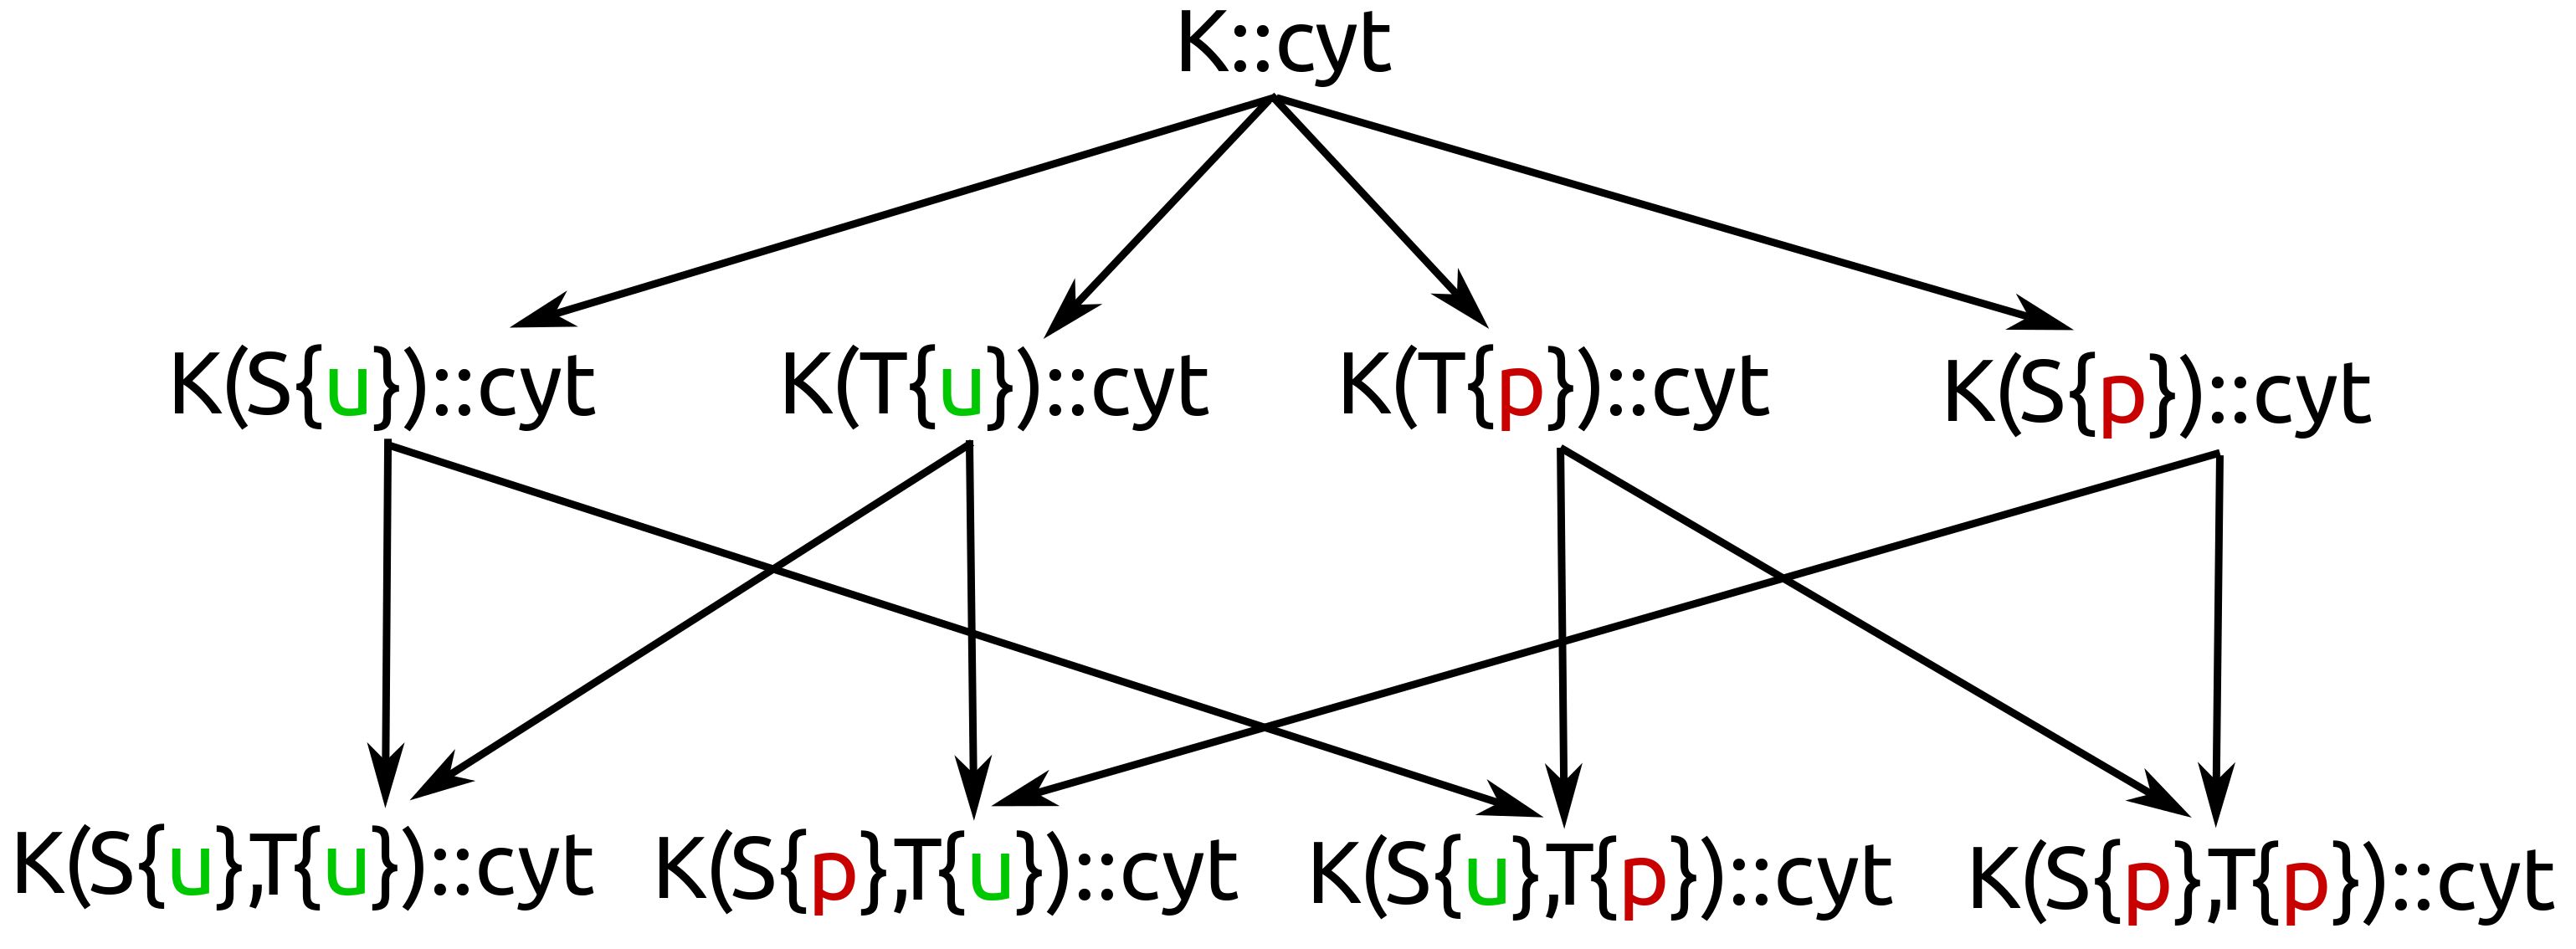
\includegraphics[scale=0.13]{pics/partial_order}
\end{center}
\caption{An example of compatible set $\mathbbmss{X}$. The partial order is depicted by a tree. For better readability, the agents are written in BCSL syntax. In this case, it is formed by a complex in $cyt$ compartment, which has only one structure agent $K$ in its sequence. The structure agent $K$ has allowed atomic agents $T$ and $S$ in its partial composition. These two atomic agents might occur in two states -- $u$ and $p$. The set is complete -- there are all relevant agents bounded by compatibility operator.}
\end{figure}

\begin{theorem}
Each agent $\mathtt{X}$ belongs to exactly one set $\mathbbmss{X}$.
\end{theorem}

\begin{proof}

[Proof by contradiction.]

Lets assume a complex agent $\mathtt{X}$ belongs to two compatible sets, namely $\mathtt{X} \in \mathbbmss{X}_1, \mathbbmss{X}_2$. From the Definition~\ref{compatible_set} condition~(\ref{compatible_cond}) follows that there exists a $\mathtt{X}_1 \in \mathbbmss{X}_1$ such that $\mathtt{X} \lhd \mathtt{X}_1$. 

Then, the condition~(\ref{non_compatible_cond}) claims that no complex agent from $\mathbbmss{X}_1$ and no complex agent from $\mathbbmss{X}_2$ can be compatible. Namely, $\mathtt{X}_1 \in \mathbbmss{X}_1$ cannot be compatible with $\mathtt{X} \in \mathbbmss{X}_2$. However, $\mathtt{X}$ and $\mathtt{X}_1$ are compatible ($\mathtt{X} \lhd \mathtt{X}_1$). It follows $\mathtt{X} \not\in \mathbbmss{X}_2$, what is a contradiction. $\QEDA$

% via identity?
\end{proof}

Practically, relation following from compatibility operator can be used in several ways. It is suitable for deeper static analysis on level of complexes~\ref{context_reduction} and for finding nontrivial relationships between the rules~\ref{rule_redundancy}.

\begin{remark}
\label{generating_vs_compatibility}
Note that in the process generating reactions from the rules (Section~\ref{Generating reactions}), we are using ground form function (Section~\ref{ground_forms}). What the function basically does is it adds context to individual complex agents (and its substructures). In the definition of the function we provided exact procedure how to generate such agents.

However, when we look at the process more theoretically, a set of appropriate complex agents is generated for every complex agent $\mathtt{X}$ in the rule $\mathtt{R}$ and then they are connected to multiple unique reaction. These sets are actually subsets $\mathbbmss{X}_\subseteq$ of compatible sets $\mathbbmss{X}$ such that 

$$ \mathbbmss{X}_\subseteq \subseteq \mathbbmss{X}: \forall \mathtt{X}' \in \mathbbmss{X}_\subseteq: \mathtt{X}' \lhd \mathtt{X}$$

where $\mathtt{X} \in \mathbbmss{X}$.

\end{remark}

\subsection{Rule redundancy elimination}
\label{rule_redundancy}

There might be cases when there are redundant rules defined in a model. This might be done for example by inattention of modeller in combination with high level of abstraction language uses. These rules do not cause any semantical difference, but might slow down dynamic and/or static analysis, eventually affect the results of analysis.

\begin{theorem}

Lets have two rules $\mathtt{R}, \mathtt{R}'$ of form:

$$ \Gamma_1 + \Gamma_2 + \ldots + \Gamma_n \Rightarrow \Gamma_{n+1} + \Gamma_{n+2} + \ldots + \Gamma_{m} $$

for some $m,n \in \mathbb{N}$ such that both $\mathtt{R}, \mathtt{R}'$ are well-formed rules.

We declare rule $\mathtt{R}$ as a \emph{redundant} rule iff

$$ \forall i \in [ 1, m ]: \mathtt{F}(\Gamma_i) \lhd \mathtt{F}(\Gamma'_i). $$
\end{theorem}

In other words, the rule $\mathtt{R}$ does not add any semantic details or the rule itself has no effect.

-- add an example

For the proof we can use compatible sets of complex agents $\mathbbmss{X}$ and the fact that when we are generating reactions from rules, we are actually enumerating all agents from the set $\mathbbmss{X}$ which are \emph{compatible with} original agent in the rule (Remark~\ref{generating_vs_compatibility}).

\begin{proof}
The problem whether the elimination of redundant rules preserves semantics can be reduced to a simple question -- if it holds for single pair of complex agents for a position $k$ in the rules, then it generally holds for entire rule.

The complex agents $\mathtt{X}_k = \mathtt{F}(\Gamma_k)$ and $\mathtt{X}'_k = \mathtt{F}(\Gamma'_i)$ both belong to the same compatible set $\mathbbmss{X}$ since $\mathtt{X}_k \lhd \mathtt{X}'_k$, which follows from the condition of the theorem. 

Then, we can create subsets $\mathbbmss{X}_\subseteq, \mathbbmss{X}'_\subseteq \subseteq \mathbbmss{X}$ for both complex agents respectively (Remark~\ref{generating_vs_compatibility}). Because the agents are compatible ($\mathtt{X}_k \lhd \mathtt{X}'_k$ ), the compatible subset $\mathbbmss{X}_\subseteq$ of agent $\mathtt{X}_k$ is either subset or equal to set $\mathbbmss{X}'_\subseteq$ of agent $\mathtt{X}'_k$:

$$\mathbbmss{X}_\subseteq \subseteq \mathbbmss{X}'_\subseteq.$$

Therefore, the produced set of reactions from the redundant rule is actually a subset of reactions produced from the non-redundant rule. $\QEDA$
\end{proof}

\subsection{Context-based reduction}
\label{context_reduction}

Reduced model $\widetilde{\mathds{M}}$ is created form given BCSL model by reducing context of complexes in rules to maximum level. This is achieved by taking supremum from compatible set $\mathbbmss{X}$. This procedure might produce rules with no action, i.e. not well-formed rules -- such rules might be omitted. Then, only rules creating/destroying agents and complex formation/dissociation should remain, providing reduced network. Since we are reducing context, the resulting network can be equal or smaller than the original one.

\begin{definition}{Reduced model}
\label{reduced_model}
Reduced model $\widetilde{\mathds{M}}$ is a pair $(\widetilde{\mathcal{R}}, \widetilde{\mathtt{init}})$ where $\widetilde{\mathcal{R}}$ is set of rule expression and $\widetilde{\mathtt{init}}$ is initial multiset of complex agent expressions constructed from given BCSL model $\mathds{M} = (\mathcal{R}, \Sigma_\mathtt{A}, \Sigma_\mathtt{T}, \mathtt{init})$ such that the following condition holds:

\begin{enumerate}
	\item for every rule $\mathtt{F}(\widetilde{\rho}) = (\widetilde{\chi}, \widetilde{\omega}, \widetilde{\iota}, \widetilde{\varphi}, \widetilde{\psi}) \in \mathds{R}$ such that $\widetilde{\rho} \in \widetilde{\mathcal{R}}$ and appropriate original rule $\mathtt{F}(\rho) = (\chi, \omega, \iota, \varphi, \psi) \in \mathds{R}$ such that $\rho \in \mathcal{R}$ holds:

	$$\forall i \in [1, k]: \pi_i(\widetilde{\chi}) \equiv \mathtt{sup}(\mathbbmss{X})$$ where $\mathbbmss{X}$ is a compatible set such that $\pi_i(\chi) \in \mathbbmss{X}$,

	\item for every complex agent $\widetilde{\mathtt{X}} = \mathtt{F}(\widetilde{\Gamma}) \in \widetilde{\mathtt{init}}$ and appropriate original complex agent $\mathtt{X} = \mathtt{F}(\Gamma) \in \mathtt{init}$ the following condition holds:

	\begin{center}
	$ \widetilde{\mathtt{X}} \equiv \mathtt{sup}(\mathbbmss{X}) $ such that $\mathtt{X} \in \mathbbmss{X}$
	\end{center}

\end{enumerate}

where length $k$ of each pair of rules $\mathtt{F}(\widetilde{\rho}$) and $\mathtt{F}((\rho)$ is equal (i.e., number of complex agent expression is the same on both sides).

Moreover, all rules which are not well-formed are removed afterwards.
\end{definition}

A reduced model $\widetilde{\mathds{M}}$ is actually an over-approximation of an BCSL model $\mathds{M}$. Therefore it can be used for some analyses, which would avoid combinatorial explosion of the original model.

\begin{theorem}
\label{non-reachability_in_reduced}
We want to check whether an complex agent $\mathtt{X}$ is non-reachable in the LTS of a given BCSL model $\mathds{M}$. Let $\mathbbmss{X}$ be a compatible set for $\mathtt{X}$.

If supremum $\mathtt{sup}(\mathbbmss{X})$ is non-reachable in reduced model $\widetilde{\mathds{M}}$ constructed with respect to given model $\mathds{M}$, then agent $\mathtt{X}$ is also non-reachable in the LTS of the original model $\mathds{M}$.
\end{theorem}

If we are checking whether an agent is reachable for given model $\mathds{M}$, we might first check whether its super-ancestor is reachable in created reduced model $\widetilde{\mathds{M}}$. If so, then we are still not certain about reachability of agent itself and it has to be checked in the original model. However, when it comes to non-reachability (Theorem~\ref{non-reachability_in_reduced}), agent which is non-reachable in $\widetilde{\mathds{M}}$ is not reachable in the original model $\mathds{M}$ too.

\begin{proof}

[Proof by contradiction.]

Lets assume a complex agent $\mathtt{sup}(\mathbbmss{X})$ is non-reachable in LTS of reduced model $\widetilde{\mathds{M}}$, but $\mathtt{X} \in \mathbbmss{X}$ is reachable in LTS of the given model $\mathds{M}$.

Generally, there is a path formed from rules in the original LTS such that we transform complex agents from initial agents to desired complex agent $\mathtt{X}$. However, once we move to context of reduced model $\widetilde{\mathds{M}}$, there is no such path for $\mathtt{sup}(\mathbbmss{X})$. However, according to Definition~\ref{reduced_model}, for every such rule there exist a reduced rule, such that all interacting complexes are reduced to their supremas. Therefore, if we could apply a original rule on a complex agent, we can do the same with reduced rule and its supremum. It follows there must exist such path also in reduced LTS and the complex agent $\mathtt{sup}(\mathbbmss{X})$ is reachable, what is a contradiction. $\QEDA$
\end{proof}

This approach can be generalised for non-reachability of a (multi)set of complex agents, but we consider it as a future work.

\subsection{Static reachability analysis}

Since we have defined compatibility operator for agents, we can apply static reachability analysis before enumerating whole state space of the model $\mathds{M}$. This analysis has its limitations, but can serve for checking whether a complex agent $\mathtt{X}$ is non-reachable (similarly as in the previous section). For that, all we need is set of rules $\mathcal{R}_f$ created from set of rule expressions $\mathcal{R}$ of model $\mathds{M}$ with semantic function $\mathtt{F}$.

\begin{theorem}
\label{static_reach}
We can declare a complex agent $\mathtt{X}$ as non-reachable w.r.t. set of rules $\mathcal{R}_f$ iff there does not exist a rule $\mathtt{R} = (\chi, \omega, \iota, \varphi, \psi) \in \mathcal{R}_f$ such that $\exists \mathtt{X}' \in \chi: \mathtt{X}' \lhd \mathtt{X}$.
\end{theorem}

The Theorem~\ref{static_reach} states a very powerful fact in context of non-reachability analyses. Compared to dynamic non-reachability analyses, it completely avoids any combinatorial explosion and gives answer only by linear testing of structural properties of rules.

\begin{proof}
It does not matter how many rules we have to apply in order to create desired agent from the initial state. Important is that at some point on the path we have to create a complex agent $\mathtt{X}_2 \lhd \mathtt{X}$ from a complex agent $\mathtt{X}_1$ applying a rule $\mathtt{R}$. 

\begin{center}

\includegraphics[scale=0.15]{pics/static_reach}
\end{center}

In order to happen such action, there has to be at least one rule which has on its right-hand-side a complex agent compatible with the given complex agent. $\QEDA$
\end{proof}

This procedure can be extended for checking reachability of multiple complex agents, however, it does not consider stoichiometry.

\subsection{Automatic synthesis of signatures}

The BCSL model definition as given in Section~\ref{BCSl_model} can be reduced by signatures. Note we do not mean extended signatures by complex names -- just the basic signatures for atomic and structure agents. These can be obtained statically from the rules (and the initial state) linearly. The process comprises these steps:

\begin{enumerate}
\item prepare empty signature sets $\Sigma_\mathtt{A}$ and $\Sigma_\mathtt{T}$, 
\item create rule $\mathtt{R} = (\chi, \omega, \iota, \varphi, \psi)$ for every rule expression $\rho$ using semantic function $\mathtt{F}$,
\item iterate through all $\omega \in \mathtt{R}$ and:
\begin{enumerate}
  \item \label{atomic_iter} for every atomic agent $\mathtt{A}$ do the following:
  	\begin{enumerate}
  		\item \textbf{if} $\exists x \in \Sigma_\mathtt{A}: \eta(\mathtt{A}) \equiv \pi_1(x) $ 

  		\textbf{then} $\delta(\mathtt{A}) \mapsto \pi_2(y)$

  		\textbf{else} $(\eta(\mathtt{A}), \{~\delta(\mathtt{A})~\}) \mapsto \Sigma_\mathtt{A}$;
	\end{enumerate}
  \item \label{structure_iter} for every structure agent $\mathtt{T}$ do the following:
	\begin{enumerate}
	  \item \textbf{if} $\exists x \in \Sigma_\mathtt{T}: \eta(\mathtt{T}) \equiv \pi_1(x) $

	  \textbf{then} $\forall \mathtt{A} \in \gamma(\mathtt{T}): \eta(\mathtt{A}) \mapsto \pi_2(y)$ and 

	  \hspace*{1cm} do step~\ref{atomic_iter} with every atomic agent $\mathtt{A}$

	  \textbf{else} $(\eta(\mathtt{T}), \{ \eta(\mathtt{A}) ~|~ \mathtt{A} \in \gamma(\mathtt{T}) \}) \mapsto \Sigma_\mathtt{T}$ 

	  \hspace*{0.75cm} (also do step~\ref{atomic_iter} with every atomic agent $\mathtt{A}$).
	\end{enumerate}
\end{enumerate}
\end{enumerate}

We could discuss fact that desired signature might be in some manner \emph{bigger} than the collected ones. However, if for example we want to have more states defined for an atomic agent, they should be definitely used somewhere in the model. In other case, it does not play any role in the model behavior and therefore its definition is senseless. In other words, the described procedure guarantees collecting all signature details which play any role in the model.

% \begin{proof}
% Let $\mathcal{M}$ be a BCSL model and $\Sigma$ its minimal signatures (i.e., all states and partial compositions defined in the signatures are actually used in the rules). Then, signatures $\Sigma'$ obtained by procedure (ref blah) has to be equal to the original signature $\Sigma$. In case its not, it means either there is some extra data in the $\Sigma'$ or some data is missing. Since we create $\Sigma'$ by iterating through all the rules, we construct complete signature with complete states used in the model. Therefore, if some data are missing in $\Sigma'$, then it follows given signature $\Sigma$ is not minimal. On the other hand, if there are some extra data in $\Sigma'$, then given signature $\Sigma$ is incorrect -- its missing some structure details which are being used in the model. $\QEDA$
% \end{proof}

\subsection{Minimal optimal bound of the system}
\label{optimal_bound}

Transition systems produced by semantics of BCSL models are infinite in general. Despite the fact the underlaying reaction networks are always finite (Section~\ref{optimal_bound}), there are types of reactions which can increase number of occurrences in a state with no limitations. Typically, such reactions form interface between the modelled system and the environment.

However, the process of applying vector reactions on states can be extended by a control system. This system does not allow to grow individual values inside the state vector above given bound. Simply, if produced vector should obtain an integer higher than the bound, the action is not taken. This procedure is very similar to checking whether all values in the vector are positive.

The only remaining issue is what is an optimal value for the bound. The universal solution is to let the modeller decide. It follows extension of model definition by the bound. However, this process requires the user to know additional information about the model and additional effort. It does not fit to purposes of the language.

Therefore we decided to apply a static analysis on the model. We will not provide a formal definition of this analysis, rather give intuition and reason about this particular solution.

We decided to find a minimal bound, which is in this context optimal for generating all required objects. It means that all the complexes which are potentially encoded in rules (reactions) will be produced, but only in one repetition. In other words, with this bound a minimal network should be created. In such network, every agent reachable in boundless network is reachable also in minimal network.

To actually calculate the minimal bound, we take maximum value from the following measurements:

\begin{itemize}
  \item count the highest number of occurrences from all agents in initial state,
  \item count the highest number of unique agents in all complexes of all rules,
  \item count the highest stoichiometry in all left- and hand-sides of the rules.
\end{itemize}

This should guarantee that it is possible to achieve high enough number of occurrence to produce any complex or combination of complexes.

\subsection{Translation to Petri Net}

By generating reaction-based model from rule-based, which is always possible (Section~\ref{Generating reactions}), we can furthermore translate such model to Petri Net~\cite{petri}.

definition of petri net goes here

The translation is quite straight-forward: 

\begin{enumerate}
\item as described in (section XY), we have finite number of unique agents -- these are all the places \emph{p}
\item transitions \emph{t} are constructed as follows:
\begin{itemize}
  \item for each reaction, create a transition,
  \item place input edge from each place which has label in left-hand-side of the rule (with appropriate multiplicity),
  \item do the same for output edges for right-hand-side of the rule,
\end{itemize}
\item finally, we create initial marking \emph{m} from given initial state of the model by similar procedure described above.
\end{enumerate}

Once the model is translated, we are allowed apply all available analysis which are provided by Petri Nets. For example, P and T invariants, deadlock detection, coverability etc. (see~\cite{petri}).

\chapter{Implementation}

In order to support usability of the BCSL language, we developed software tool BCSgen. The general goal of the tool is to provide environment suitable for editing and maintenance of the BCSL models and provide functionality to analyse the models. The software was developed in several iterations. Firstly as independent project MUNI33/092015 in \emph{Dean's Program of the Faculty of Informatics MU for support of student research and development projects}, later as part of the project MUNI33/062017 in the same program. Finally, it was finalized to current stage in this thesis.

The tool is developed in Python language (version 2.7) as open-source desktop software build under GPL-3.0 license. The source codes, short tutorial for usage and installation, and current stable version as binary files are available on GitHub\footnotemark[1]\footnotetext[1]{\url{https://github.com/sybila/BCSgen}}.

In the first iteration, there was no support for models editing. The only functionality provided by the tool was import of the model from a text file (in particular format) and enumerating whole state space of the model. Moreover, the implementation was done by translating to Kappa and it was rather slow and non-efficient. The single transaction (application of one rule) was delayed by translation to Kappa and then by exact matching and replacement, which might get quite complicated. However, it was a good start for the language and it was possible to analyse exported networks in external tools. There was simple GUI made in Tkinter~\cite{Tkinter}, which had several issues. The most important one was the fact that Tkinter was not designed for multithreading programming. Therefore, for example, while computing a state space for the model, the whole GUI was not responsible.

In the second iteration, we focused on speed improvement and development user-friendly GUI. For the speed improvement, we implemented semantics as defined in this thesis (Section~\ref{semantic_function}). Compared to previous iteration, now there was no exactly rule-based execution of the rule -- rules we rather translated to reactions and subsequently encoded as vector operations over integers. Therefore, one transaction was just addition of one vector (left-hand-side) and subtraction of another one (right-hand-side). The GUI was reimplemented in PyQt~\cite{summerfield2007rapid}, which naturally works with multithreading. In this area, it was huge step forward. Moreover, we improved input/output formats. For input, we defined BCSL model format, which serves for import. As output format we have chosen JSON, which is very suitable for its simplicity and support by many external tools.

In the last iteration, which is part of this thesis, we focused on improvement of models maintenance, additional analysis services, and visualisation. We have integrated editor which is able to highlight syntax errors while building the model. To achieve this, we needed an efficient rule-parser which would be able to parse the rules very fast. The parser is able to parse even syntactic extensions defined in Section~\ref{syntactic_extensions}. The rules engine then translates the rule to ground form and creates reactions (in case there are no errors in the model). Since this engine runs in the background (in another thread) user does not notice any increased performance. Once reactions are computed, this is indicated by possibility to export them and generate state space of the model.

Next, we implemented additional analysis. Namely, model simulation and reachability analysis. For the simulation, we allow stochastic or deterministic form. In the first one, random rules are fired according to Poisson distribution while in latter average trace is computed by solving ODEs build from the reactions. For the stochastic case, there are options to choose number of runs and apply interpolation on resulting time series chart in order to achieve smoother results. It is important to note that only models with defined rates can be simulated. For simplicity, approach where only fully specified agents are used (Section~\ref{rates_discussion}) was chosen from the discussed ones.

 -- more info about static analysis goes here

Since there are some graphs and charts generated in BCSgen, we decided to integrate visualisation tools into it. For this, we used two libraries -- vis.js~\cite{almende2016vis} for interactive networks visualisation and MatPlotLib~\cite{hunter2007matplotlib}, a Python library suitable for visualisation of time series. Vis.js is used for exploration of state space with highlighting chosen node and announcing content of the node. Moreover, it is possible to display paths from initial state to other states, which satisfy reachability condition given in reachability analysis part. This is very demonstrative and suitable for education purposes. However, such visualisation has its limitations, for huge graphs its very difficult to display the graph -- on the other hand, from such number of nodes it is not even useful. The MatPlotLib provides visualisation of simulation results. It possible to zoom the chart, hide/show individual curves, and export the current view as a picture.

As a future work for the tool we are planning to reimplement it to a web-based version. In ideal case, it should be integrated to CMP (Section~\ref{cmp}) to allow direct analysis of the models and appropriate parts of Biochemical Space.  

\chapter{Case study}
\label{case_study}

To demonstrate Biochemical Space has practical use, we introduce an instance of CMP, where BCS is used in practice. E-cyanobacterium.org~\cite{Trojak2016} is an online platform providing tools for public sharing, annotation, analysis, and visualization of dynamical models and wet-lab experiments related to cyanobacteria. The general aim is to stimulate collaboration between experimental and computational systems biologists to achieve better understanding of cyanobacteria. As an instance of CMP, it covers all the features of the platform.

The following processes of cyanobacteria are covered in BCS: environmental processes, respiration and photosynthesis, carbon concentrating mechanism, circadian clock, and metabolism. Currently, the repository of models contains two models describing circadian clock (Miyoshi et al. 2007~\cite{Miyoshi01022007}, Hertel et al. 2013~\cite{Hertel2013}) and a kinetic model of metabolism (Jablonsky et al. 2014~\cite{Jablonsky2014}). Two other models present unpublished results -- dynamics of carbon fluxes (M\"{u}ller et al.) and photosynthesis (Plyusnina et al.). Additionally, two models in development describing carbon concentrating mechanism are Clark et al. 2014~\cite{clark2014insights} and Fridlyand et al. 1995~\cite{fridlyand1996quantitative}. Each of them was properly mapped on the BCS and helped to form suitable space covering all the mentioned processes.

Entire biochemical space of cyanobacteria is formed from over 1000 entities and 600 rules. Therefore, we will not explain them all here, we just provide a several cases which demonstrate how different BCSL features can be used for describing real biological problems.

The circadian clock of cyanobacteria~\cite{CCR} is formed by three kinases KaiA, kaiB, and KaiC (with additional presence of ATP). The key role plays KaiC. Compared to the other two proteins, it is physically the biggest one. As every protein, its primary structure is a sequence of amino acids, where two particular are important for the modelling -- threonine and serine. These two amino acids can be enriched by phosphoryl group in process commonly known as phosphorylation~\cite{cohen2002origins}. However, the sites are accessible only when the protein forms a homohexamer -- a structure of six KaiC proteins. For the phosphorylation itself are responsible KaiA proteins while KaiB proteins inactivate KaiA's, which leads to auto-dephosphorylation of KaiC kinases. There are several complexes which can be formed from mentioned proteins according to situation which is currently happening with the KaiC hexamer.

It is important to note the KaiA and KaiB kinases only \emph{enhance} the phosphorylation process, but do not enable/disable it completely. Therefore, when it comes to quantitative description of the system, it is necessary to depict all possible actions. Particularly, we need to express the fact the phosphorylation process happens regardless the complex KaiC hexamer is currently in. 

-- phosphorylation example rule goes here

Another interesting aspect of the circadian clock is formation of KaiC hexamers. The condition that a KaiC protein can be (de)phosphorylated \emph{only} inside a hexamer leads to one important fact -- it does not mean the hexamer must be assembled from/dissociated to unphosphorylated KaiC proteins. The hexamer can be dissociated at any point in time, for example when three KaiCs are phosphorylated on the serine residue, other two are phosphorylated on both residues, and the last one is not phosphorylated. It is quite obvious the number of possible combinations is quite huge. But still we need to describe this fact in the system we are modelling.

Fortunately, rule-based languages including BCSL are very suitable for such cases. What we actually need to express is situation, when a complex needs to be formed (or dissolveed) regardless the context (states) of the interacting entities (six KaiC proteins).

-- kaic formation rule goes here

Another interesting process inside cyanobacteria is photosynthesis. It is performed on internal membranes called thylakoids. In general, photosynthesis in cyanobacteria uses water as an electron donor and produces oxygen as a product. Electron transport is performed though multiple protein complexes, which together form the thylakoid membrane itself. Such complexes are for example photosystem I. and II. However, model the complexes directly is not very efficient. The typical rules in photosynthesis are just electron transfers between the complexes or reduction/oxidation of individual parts. Therefore, such action usually happen regardless the context of the rest of the complexes in a photosystem. The best approach with respect to BCSL language is to usage structure agent for defining the protein complexes and its individual parts model as partial composition.

-- example rule ID 4 and 33 

it would be great to somehow demonstrate defined statical analysis here

-- could be defined a small model with question of reachability of some agent, which can be answered directly without enumerating state space

-- also the context reduced network -- a more complicated model which is small after reduction, show that something is not reachable

practical examples of defined objects

\chapter{Discussion}

\subsubsection{The difference between BCS and BCSL}

It is important to realise the difference between Biochemical Space and Biochemical Space Language which we are about to define.

The general goal of BCS is to provide knowledge base for mathematical models. In order to achieve that, Biochemical Space is formed by a database of biochemical entities. This allows us to describe particular objects with their attributes and properties and form space hierarchy. Each entity should be properly annotated by description and links to suitable external databases. However, entities are not enough for describing models since it requires also process hierarchy. Therefore, alongside with space hierarchy of entities, process hierarchy is build via interactive schemes. The hierarchy allows us to zoom on individual rules which present atomic operations happening on the entities.

To improve usability and verifiability of the BCS, we define Biochemical Space Language. The language formally describes the entities and the rules. It has rule-based semantics, what allows compact description of the objects. Moreover, the syntax was designed in order to be very concise and human-readable. Hence it is very suitable for our needs.

The whole BCS is defined in BCSL. This fact makes sure the entities and the rules are defined with all appropriate properties. Moreover, it helps us to relate objects from the models to BCS objects. Note that due to rule-based nature of the BCSL, in BCS there are defined only abstract objects representing types. Therefore, when relating for example an model variable to BCS entity, we might need to specify its properties. 

\begin{figure}[!h]
\begin{center}
  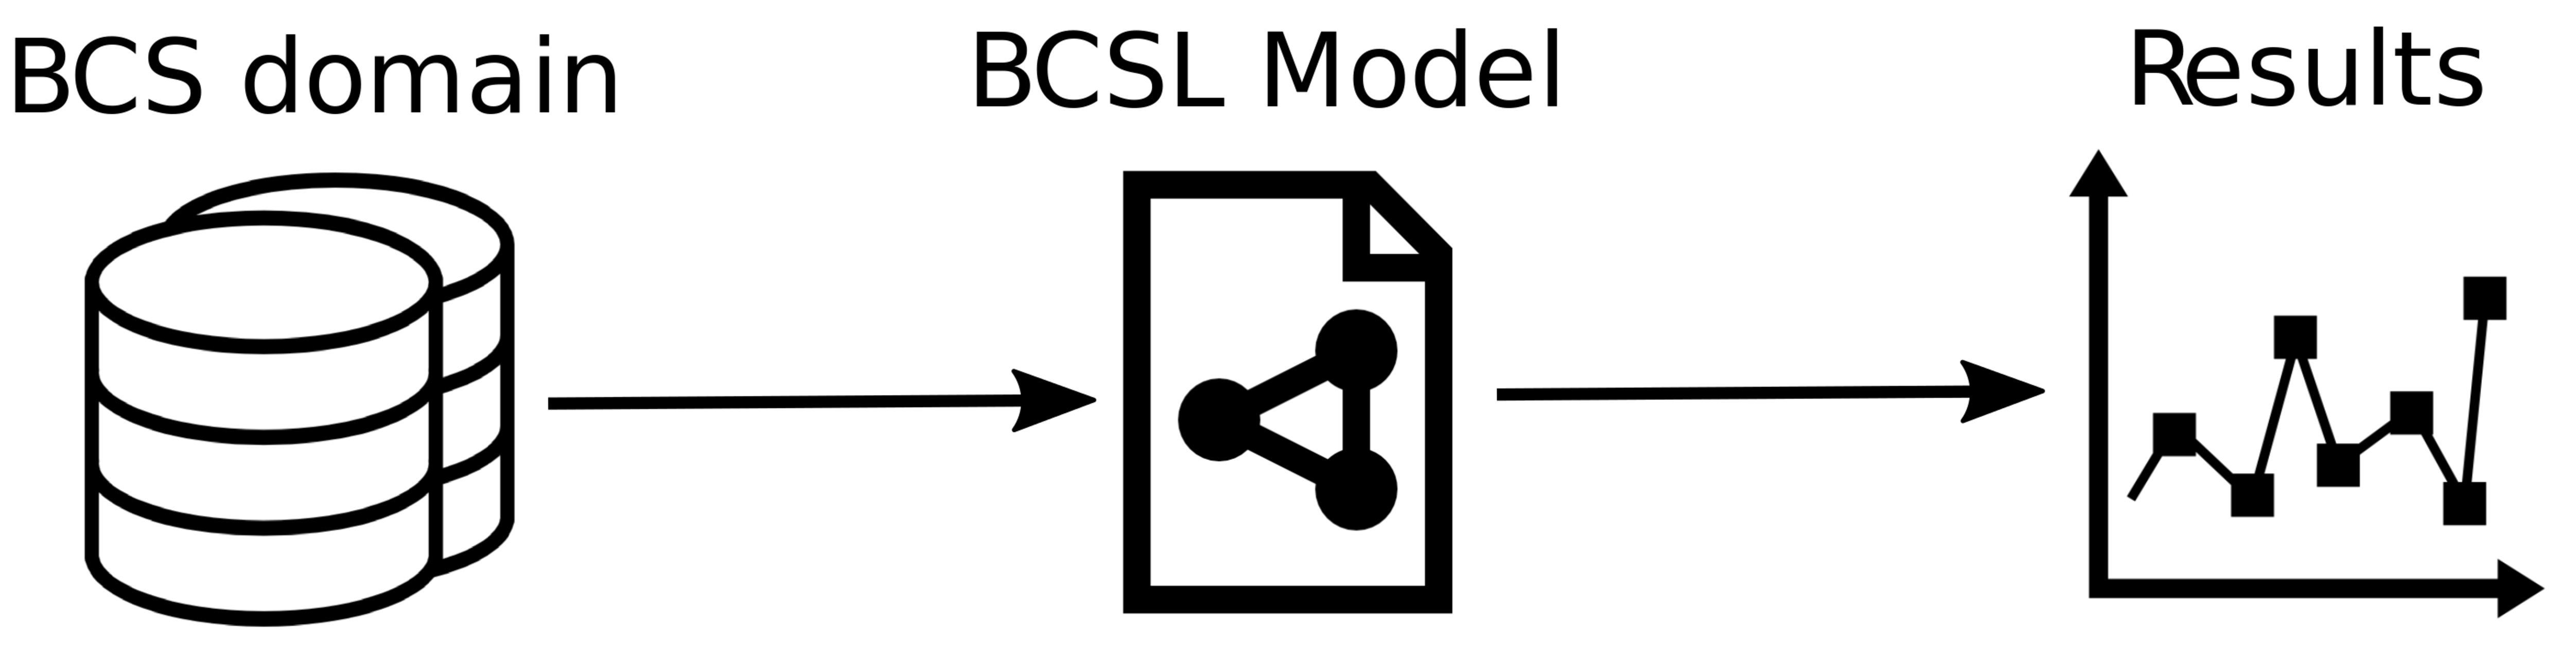
\includegraphics[scale=0.13]{pics/bcsl_vs_bcs.pdf}
\end{center}
\caption{BCS domain serves for improved BCSL models definition, which leads to better model readability and results.}
\end{figure}

Once BCS is build, we can use it to reference the models. It means to relate all the variables and reactions of the model and to entities and rules of BCS. In particular, each variable should have assigned an entity for BCS. It increases information value of the variable (due to annotation of BCS entity). Since reactions of the model are composed from its variables, this way we also rewrite general reactions to reactions written in BCSL. The result of relating all the entities is model written in BCSL. 

Model defined in BCSL has two main advantages -- formal analysis can be applied on the model and the biological meaning of the whole model is fully reconstructed.

To sum it up, BCS serves as definition domain for models written in BCSL (so called signature). It defines what can and what cannot be written in models and also increases rule compactness due to syntactic extensions. For example, some context might be omitted from the rule because it can be reconstructed from the signature.

\chapter{Conclusions}

\bibliographystyle{citeStyle}
\bibliography{papers}

\appendix

\chapter{Cheat sheet}

\begin{tabular}{c c | l}
$\sigma(\vv{v})$ & & set of permutations of vector $\vv{v}$ of length $|\vv{v}|$\\
$\Sigma_{\mathtt{A}}$ & & atomic signature \\
$\Sigma_{\mathtt{T}}$ & & structure signature \\
$\mathtt{A}$ & & atomic agent \\
 & $\eta$ & name \\
 & $\delta$ & state \\
 & $\varepsilon$ & empty state (not specified)\\
$\mathds{A}$ & & universe of all possible atomic agents \\
$\mathtt{T}$ & & structure agent \\
 & $\eta$ & name \\
 & $\gamma$ & partial composition\\
$\mathds{T}$ & & universe of all possible structure agents\\
$\mathtt{X}$ & & complex agent\\
 & $\mu$ & sequence of agents\\
 & $\mathtt{com}$ & compartment\\
$\mathds{X}$ & & universe of all possible complex agents\\
$\mathds{U}$ & & universe of all possible agents\\
$\mathtt{R}$ & & rule\\
 & $\chi$ & sequence of complexes\\
 & $\omega$ & sequence of atomic and structure agents\\
 & $\iota$ & index determining start of right-hand-side\\
 & $\varphi$ & index map between $\omega$ and $\chi$\\
 & $\psi$ & is an index map between agents from left-\\
 & & and right-hand side\\
$\mathds{R}$ & & universe of all possible rules\\
$\mathtt{r}$ & & reaction\\
 & $LHS(\mathtt{r})$ & left-hand-side of the reaction\\
 & $RHS(\mathtt{r})$ & right-hand-side of the reaction\\
$\alpha$ & & atomic expression\\
$\tau$ & & structure expression\\
$\Gamma$ & & complex expression\\
$\rho$ & & rule expression\\
$\mathds{M}$ & & BCSL model\\
 & $\mathcal{R}$ & set of rule expressions\\
 & $\mathtt{init}$ & initial multiset of complex expressions\\
\end{tabular}

\begin{tabular}{c c | l}
$X \mdoubleplus Y$ & & tuples concatenation\\
$\mdoubleplus_{i=1}^n T_i$ & & generalised concatenation\\
$\pi_i$ & & projection on dimension i\\
$\mathtt{reassembly}(Y)$ & & reassembly of tuples\\
$\gamma \ominus \gamma'$ & & difference of partial compositions\\
$\Sigma_T(\mathtt{\eta(\mathtt{T})}) \ominus \gamma(\mathtt{T})$ & & difference of partial composition and\\
 & & structure signature\\
$\mathtt{F}$ & & semantic function\\
$\mathcal{G}$ & & ground form function\\
$\mathcal{M}$ & & Chemical Reaction Model\\
 & $\mathfrak{R}$ & set of chemical reactions\\
 & $\vv{\nu}$ & initial vector\\
 & $\theta$ & vector of reference complexes\\
$\varrho$ & & chemical reaction application\\
$\mathtt{S}$ & & a multiset of agents\\
$\lambda(\mathtt{S}, \theta)$ & & multiset to vector translation\\
\end{tabular}

\chapter{Discussion about rates and how they could be solved}
\label{rates_discussion}

In order to provide numerical simulation, we need to assign a reaction rate to each rule. However, this is quite a challenging task and we will briefly explain why.

The general problem is that typical kinetic rules in biology require usage of concentration of an agent in volume of the system. This is often solved via absolute numbers (the number of repetitions). The number might be either natural number of we are working with stochastic simulation or even real number if we compute average traces such as in deterministic simulation (make this more precise with citations!!!).

Compared to reaction-based models, we work with fully defined objects which we can simply reference in the kinetics without any limitations. We can do the very same in rule-based models, but it is not desired solution. The thing is we would like to express the context of the rule also in the kinetics. That typically means when context in which the rule is being applied changes, we want appropriate change in the kinetics. To make this more clear, we provide an example.

Example goes here...

There are several solutions of this problem. However, none of them is an optimal one and therefore this remains an open problem. In other languages... they solved it as... finish this...

Another general problem which causes issues is stoichiometry. The problem is if we reference an agent which has multiple enumerations in the rule, it is not clear which one should be used as reference in kinetics. Therefore we distinguish two types of solutions:

\textbf{Solutions with forbidden stoichiometry}:

\begin{enumerate}
\item unique agents

In this case, we allow arbitrary kinetics, but with a restriction. It is not allowed to use two identical agents in the same rule (including both sides of the rule). Moreover, in kinetics it is allowed to use only agents which are already used in the rule (in the very same form). This restriction decreases the expressiveness of the rules -- for example, it is not possible to define agents which are required but not consumed in the rule. However, mapping between agents in rule and kinetics are clear.

\item almost optimal solution

In order to make sure the agent from kinetics and rule are connected properly, we would have to extend the syntax of the language itself. For example, and agent might be enriched by `$\sim\mathbb{N}$' in both places. Then, the mapping would be unambiguous. However, such s syntax extension leads to decreases readability of the language, which definitely not desired solution. Optionally, the numbering of agents might be implicit, what does not change syntax of the language, but makes it harder to write w.r.t. language simplicity.

\end{enumerate}


\textbf{Solutions with allowed stoichiometry}:

\begin{enumerate}
\item we allow only \emph{mass action} kinetics

The positive thing about this kinetics is that all it needs is a given parameter. The rate is computed as multiple of the parameter with all agents on the left-hand-side of the rule. Since the stoichiometry is allowed in this case, the mapping is not always clear. For this reason we multiply all possible mappings together, which gives appropriate results.

\item the first left agent

Arbitrary kinetics might be used, but both rule and kinetics must be defined very carefully. The method for mapping rate agent to rule agent is very simple -- whenever an agent is referenced in kinetics, first suitable rule-agent from the left is chosen. This solution is very simple to use, but rules are not that easy to write.

\end{enumerate}

\end{document}
